\documentclass{article}

% Use custom style
\usepackage{mystyle}

% Use Reference table
\addbibresource{references.bib}

% Use Acronym table
\loadglsentries{glossary.tex}

% Use title
\title{TTK4551 Technical Cybernetics - Specialization Project}
\author{Martynas Smilingis}
\date{September 2025}

% Document (START) ==================================================
\begin{document}

% Generated title
\maketitle

% Generate content page
\newpage
% Tabe of context
% Teporarily group table of context to make its links black instead of like the rest of the text where it is blue
\begingroup
    \hypersetup{linkcolor=black}
    \tableofcontents
\endgroup
\newpage

% Generate Acronym table and include all main glossary entries even if unused
\printglossary[type=\acronymtype, style=acronymStyle]
\printglossary 
\glsaddallunused[\acronymtype] \clearpage

% Main meat n potaters of the report
\section{Introduction}
\subsection{Goal}
\todo{TAP: The thesis is already starting to get long. At Marine Department, they have a limit of approx 80 pages for a master thesis (excluding appendices and references). We are now talking about a pre-project. Discuss this with Damiano, I'm not sure about Cybernetics, but anyway, when comming to the master thesis, being precise and concise will be key.}
\todo{TAP: Goal and motivation are natural in the introduction chapter, but not sure if Side Scan chapter is? In addition, this chapter should include some background (possible together with motivation), objectives (possible together with goal), contributions, structure of the thesis.  Have a look at other master thesis for inspiration.}
\todo[inline]{Maybe I should resturcture the Introduction Goal and Motivation maybe?...}
\todo[inline]{Also add the FN bærekrafts mål I suppose?...}
\noindent
This specialization project focuses on navigation and Simultaneous Localization and Mapping (SLAM) for marine robots, with an emphasis on Side Scan Sonar based SLAM. The main objective is to study, reimplement, and optimize the core components of modern SSS SLAM pipelines to achieve real-time performance on real world AUV datasets, such as those collected from NTNU's AUR Lab platforms (for example LAUV Harald). 
\\ \\
The work builds upon the 2023 masters thesis by Haraldstad \cite{side_scan_sonar_master_thesis} and recent research on side scan sonar landmark detection \cite{side_scan_sonar_paper}, which are heavily inspired by the earlier work of Hogstad, Bjørnar Reitan \cite{side_scan_sonar_master_thesis_old}. The projects scope is to implement and benchmark the essential components required for real-time SSS SLAM operation, validate them on existing datasets, and demonstrate that the processing pipeline can operate at or above the sonars frame rate while maintaining high mapping accuracy.
\\ \\
A second phase of the project focuses on embedded deployment on a autonomous surface vessel (ASV). The goal is to port and integrate the validated core pipeline on ship borne hardware, assess side scan sonar performance in coastal waters, and shift the work from algorithm design to practical system integration. This phase will use NTNU's MicroAmpere ASV.



\subsection{Motivation}
Reliable maritime navigation requires onboard estimation and mapping when external positioning is weak or unavailable. This project focuses on side scan sonar based simultaneous localization and mapping, SSS SLAM. SSS SLAM uses side scan sonar to estimate the vehicle pose while building a seafloor map at the same time. In SSS SLAM, sonar images drive feature extraction and data association, loop closures correct drift, and the SLAM back end fuses all measurements into a consistent trajectory and map. Marine robots operate with limited access and often far from support. They must know where they are and what surrounds them to move safely and do useful work. Static charts help, but the ocean changes over time. Currents, waves, moving vessels, new structures, and shifting seabeds make static maps go out of date. GNSS is weak or unavailable underwater, and dead reckoning drifts. Even in coastal areas, terrain can block signals, and shallow water operations require safe margins to the bottom. These factors make SSS SLAM a practical path to robust navigation and mapping.
\\ \\
Prior work \cite{side_scan_sonar_master_thesis} presented a pipeline for SSS SLAM but did not reach real time performance. Field deployment needs real time operation on real data with measured accuracy and robustness. The first motivation is to deliver a lean real time SSS SLAM implementation and to quantify performance on the same dataset used previously, so the results are directly comparable.
\\ \\
The second motivation is to move from offline studies to reliable system behavior at sea. The plan is to measure accuracy, robustness, and runtime on recorded AUV data, then prepare the pipeline for embedded use on a autonomous surface vessel (ASV). This shifts effort from algorithm design to practical integration on real hardware, including time synchronization, calibration, and stable runtime.


 \clearpage
\subsection{\gls{SSS SLAM} Architecture}
SOme images here of basic overvies
\\ \\
Talk abit on SLAM
\\ \\
Then a picture of complex overview
\\ \\
Talk a bit more in depth on slam \clearpage

 \clearpage
\section{Sonar Theory}

Talk about acoustics

Talk about Sonar

Talk about camera and visual odometry stuff and how sonar is used
 \clearpage
\section{Hardware}

Start by intro about AUV and ASV explanation
That AUV data for building up the front end and backend and test with some data to verify that the algorithms work
Then use this built up ssystem to mold and modify and optimize for ASV

Talk about AUV specs 
AUV sensors as well
AUV Data set that it was collected

Then talk about ASV specs
ASV sensors that are important
Then talk a bit about ASV software pipeline \clearpage
\section{System Modeling}

Introduction that for any navigation system it works best and is built on some assumptions about the movement of the robot and the sensor used, thsi is what we call motion model f() and measurement model h(), thsi is rigid body dynamics. In adition the robot needs to know where it is in relation to itself, its sensors and the world in a coherent and efficient manner, this is rigid body kinematics.
For kinematics use the Euler represnetation as its consise and simpel and is videly used in the navigation of ships. For AUVs its more quarternion based that dominates, hwoever since we are doing only mapping euler will work as our dornes will not be maneuvering all the way. 
Even if euler angles give singularities by deciding how to repensent euler angles smrtly in standard navigation way ie NED represnetation, we can forego using quarternions wich in tehmeselves have their own cavieates. 
Never teh less we will still be using Quarternions as some sensors give our quarternions and some algorithms work better with quarternion reprensetation, because of that it is usefull to know how to handdle tem as well.
Lastly we will have SO3 and SE3 groups as the SLAM map is built using SE3 represnetation, witch is an effective way of builing Envoroemnt over large data sets and works well with rendering as it is also used a lot in computer graphics. So Lie Grpups must be dicussed here as well 

States = [pose, linear velocity, angle]

Introduction
Kinematics 
- euler
- quarternion
- lie groups, SO(3) and SE(3)
AUV modelling
- Motion f()
- Measurents h()
ASV modelling
- Motion f()
- Measurents h()

 \clearpage
\section{State Estimation}

intro to it
Bayes filter
KF
EKF
UKF + Alternative Sigma Point generation for better aproximation and stability
Some other that might be uselful for later just to mention, like ESKF or UKF for system Idtentification for hydrostatic and parameters and better model aproximation. \clearpage
\section{Preintegration}
\subsection{Introduction}
In graph based SLAM, the preintegration method addresses the computational inefficiency caused by high frequency inertial measurements relative to low frequency exteroceptive sensors such as sonar. In a typical Side Scan Sonar SLAM (SSS SLAM) setup, a new sonar 2D map image is produced every few seconds at a rate of less thank 0.1 Hz, while the onboard IMU operates at several hundred hertz. If all IMU measurements were to be directly added to the factor graph as individual odometry factors by just simply using ESKF or UKF-M estimate, this would result in hundreds of redundant nodes between consecutive 2D sonar map frames. Such dense factor creation would significantly increase the computational load during optimization, while contributing limited additional information to the overall estimation process.
\\ \\
Preintegration resolves this problem by summarizing all IMU measurements between two 2D sonar map frames into a single compound odometry factor. This preintegrated factor represents the total relative motion, orientation change, and accumulated uncertainty over the integration interval, without introducing intermediate IMU states into the graph. The resulting factor provides the same essential motion constraints as full IMU integration using ESKF or UKF-M as Dead Reckoning estimate, but in a compact and computationally efficient form. This approach is particularly beneficial for SSS SLAM, where the sensor rate mismatch between the IMU and sonar is substantial.
\\ \\
The preintegration method uses the same INS motion model $f(x,u)$ as presented in Equation \ref{eq:kinematics-motion-model}, with minor modifications in how biases are handled and how the state propagation is performed. In contrast to the discrete propagation used in the State Estimation chapter described in Equation \ref{eq:state-estimation-discrete-propagartion}, preintegration assumes the accelerometer and gyroscope biases remain constant over the short integration window. This assumption simplifies the computation while retaining sufficient accuracy for most robotic applications.
\\ \\
The outcome of preintegration is a single, bias correctable odometry factor connecting two consecutive keyframes at the sonar update rate. This allows the SLAM system to maintain precise and consistent motion constraints while keeping the factor graph sparse. The approach achieves comparable accuracy to full state propagation methods such as ESKF or UKF-M but avoids the overhead associated with large numbers of intermediate factors.
\\ \\
Preintegration has been widely adopted in modern SLAM frameworks, including the Georgia Tech Smoothing and Mapping library (GTSAM), which provides dedicated classes for implementing preintegrated IMU factors discussed in later chapters of the thesis. The method was originally introduced for visual inertial odometry paper \cite{preintegration_camera_paper} and has been used in many modern SLAM problems such as for LiDAR and radar inertial fusion \cite{preintegration_radar_paper}. The same principles directly apply to sonar inertial systems, where the slow image acquisition rate makes preintegration a critical component for efficient factor graph optimization.
\begin{figure}[H]
    \centering
    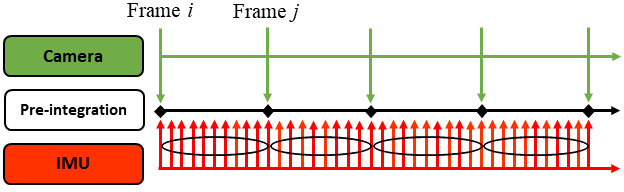
\includegraphics[width=1.0\linewidth]{Pictures/Preintegration/Introduction/Camera_IMU_example.jpg}
    \caption{Illustration of the sampling rate mismatch between an IMU and an exteroceptive sensor such as a camera or sonar. The IMU operates at hundreds of hertz, producing dense inertial measurements, while the sonar or camera generates new observations at a much lower rate. Preintegration combines all intermediate IMU readings into a single relative motion constraint that aligns with the moment a camera or sonar image is acquired.\textsuperscript{\cite{preintegration_camera_imu_picture}}}
    \label{fig:preintegration-camera-imu-example}
\end{figure}


 \clearpage
\subsection{Preintegration on Manifolds}
\subsubsection{INS Propagation Between IMU Samples}
The preintegration algorithm builds directly on the deterministic continuous time INS motion model defined in Equation \ref{eq:kinematics-motion-model}, where the system state is given by $\mathbf{x} = [\mathbf{p}_{b/O}^{n}, \mathbf{v}_{b/O}^{n}, \mathbf{q}, \mathbf{a}_b, \boldsymbol{\omega}_b]^\top$ and the input vector by $\mathbf{u} = [\mathbf{a}_m, \boldsymbol{\omega}_m]^\top$, as presented in Equation \ref{eq:kinematics-motion-model-states}. The same state representation is used here, consisting of position $\mathbf{p}$, velocity $\mathbf{v}$, and attitude $R(\mathbf{q})$, along with the accelerometer and gyroscope bias states $\mathbf{a}_b$ and $\boldsymbol{\omega}_b$. The motion model follows the same nominal kinematic equations as defined in the system modeling chapter, where the rigid body dynamics evolve according to the IMU measurements $(\mathbf{a}_m, \boldsymbol{\omega}_m)$ corrected by their respective biases. Hence, the same continuous time INS equations described in Equation \ref{eq:kinematics-motion-model} and the corresponding discrete form in Equation \ref{eq:state-estimation-discrete-propagartion} apply here.
\\ \\
In contrast to the full state estimator formulation used previously, which employed a 1st order Gauss Markov process for modeling bias drift, preintegration adopts a simpler Brownian motion bias model. This simplification is made because the preintegration window is short, and any bias evolution within this interval is small compared to the measurement noise and will be corrected later by the backend optimizer. The Brownian model is defined as
\begin{equation}
    \begin{aligned}
        \dot{\mathbf{a}}_b = \boldsymbol{\eta}_{a_b} \qquad \boldsymbol{\eta}_{a_b} \sim \mathcal{N}(0, \sigma_{a_b}^2 I_3) \\
        \dot{\boldsymbol{\omega}}_b = \boldsymbol{\eta}_{\omega_b} \qquad \boldsymbol{\eta}_{\omega_b} \sim \mathcal{N}(0, \sigma_{\omega_b}^2 I_3)
    \end{aligned}
    \label{eq:preintegration-bias-brownian-model}
\end{equation}
where $\boldsymbol{\eta}_{a_b}$ and $\boldsymbol{\eta}_{\omega_b}$ are zero mean Gaussian noise processes representing the bias random walk. The discrete time equivalent form becomes
\begin{equation}
    \begin{aligned}
        \mathbf{a}_{b,k+1} &= \mathbf{a}_{b,k} + \boldsymbol{\eta}_{a_b,d} \\
        \boldsymbol{\omega}_{b,k+1} &= \boldsymbol{\omega}_{b,k} + \boldsymbol{\eta}_{\omega_b,d}
    \end{aligned}
    \label{eq:preintegration-bias-propagartion}
\end{equation}
with $\operatorname{Cov}(\boldsymbol{\eta}_{a_b,d}) = \sigma_{a_b}^2 \Delta t I_3$ and $\operatorname{Cov}(\boldsymbol{\eta}_{\omega_b,d}) = \sigma_{\omega_b}^2 \Delta t I_3$. Over short preintegration intervals, these biases are assumed constant, meaning their change between IMU samples is negligible. The integration therefore proceeds using frozen bias estimates $\mathbf{a}_b$ and $\boldsymbol{\omega}_b$ from the start of the interval.
\\ \\
The nominal discrete time propagation of position, velocity, and rotation between IMU samples follows the same structure as the state estimation chapter in Equation \ref{eq:state-estimation-discrete-propagartion}, but is here expressed explicitly for clarity as
$$
    \begin{aligned}
        R_{k+1} &= R_k \exp([\boldsymbol{\omega}_{m,k} - \boldsymbol{\omega}_{b,k}]_\times \Delta t) \\
        v_{k+1} &= v_k + R_k(\mathbf{a}_{m,k} - \mathbf{a}_{b,k})\Delta t + \mathbf{g}\Delta t \\
        p_{k+1} &= p_k + v_k\Delta t + \tfrac{1}{2}R_k(\mathbf{a}_{m,k} - \mathbf{a}_{b,k})\Delta t^2 + \tfrac{1}{2}\mathbf{g}\Delta t^2
    \end{aligned}
$$
In this formulation, the index $k$ denotes consecutive IMU samples integrated at a high rate (typically hundreds of hertz). These samples are accumulated over the time interval between two keyframes $i$ and $j$, where each keyframe corresponds to a slower exteroceptive measurement such as a sonar 2D image frame. The goal of preintegration is to compress all intermediate IMU updates $(k=i, \ldots, j-1)$ into a single compound relative motion estimate connecting the two keyframes $i$ and $j$. 
\\ \\
The raw IMU outputs $\mathbf{a}_{m,k}$ and $\boldsymbol{\omega}_{m,k}$ represent the measured specific force and angular velocity in the body frame. The bias terms $\mathbf{a}_{b,k}$ and $\boldsymbol{\omega}_{b,k}$ are the current estimates of the accelerometer and gyroscope biases and are subtracted once within the propagation equations to obtain the corrected physical quantities. The resulting propagation is therefore already bias compensated and forms the deterministic foundation for the preintegration and subsequent error propagation steps described in the following sections.
\\ \\
At the beginning of each new preintegration interval $(t_j, t_{j+1}]$, the initial state $(R_i, v_i, p_i)$ is set equal to the optimized estimates from the previous keyframe, ie:
$$
    R_i = R_j^{\text{opt}}, \quad v_i = v_j^{\text{opt}}, \quad p_i = p_j^{\text{opt}}, \quad B_i = B_j^{\text{opt}}
$$
This ensures that the preintegration always starts from the most accurate state and bias estimates provided by the backend optimizer, maintaining temporal consistency across all keyframe intervals.



\subsubsection{Preintegration Initialization}
Preintegration is initialized at the time of keyframe $i$, corresponding to the most recent exteroceptive measurement such as a sonar frame. All IMU samples collected between keyframes $i$ and $j$ are subsequently integrated in the local coordinate frame of keyframe $i$. This ensures that the resulting preintegrated quantities describe motion relative to keyframe $i$ rather than the global frame, maintaining numerical stability and simplifying later optimization.
\\ \\
At the start of preintegration, the relative motion increments are initialized as
$$
    \Delta R_{ii} = I_3, \qquad
    \Delta v_{ii} = \mathbf{0}_3, \qquad
    \Delta p_{ii} = \mathbf{0}_3
$$
which represent, respectively, the initial relative rotation, velocity, and position between the same keyframe. These quantities form the starting point for integrating subsequent IMU samples.
\\ \\
The IMU bias used during preintegration is frozen at its current estimate from keyframe $i$, denoted by
$$
    B_i^{\text{preint}} = [\mathbf{a}_{b,i},\, \mathbf{\omega}_{b,i}]
$$
and is held constant throughout the preintegration interval $(t_i, t_j]$. The assumption of frozen bias is reasonable since the bias drift is slow compared to the short duration between keyframes, and any accumulated error is later corrected by the backend optimizer.
\\ \\
For uncertainty propagation, the Jacobians of the preintegrated quantities with respect to bias are initialized as
$$
    J_R^{\boldsymbol{\omega}_b} = J_v^{\mathbf{a}_b} = J_v^{\boldsymbol{\omega}_b} = J_p^{\mathbf{a}_b} = J_p^{\boldsymbol{\omega}_b} = 0
$$
These matrices are propagated forward with each IMU sample to capture how small bias perturbations affect the resulting preintegrated deltas, allowing efficient bias correction without re-integrating all IMU data.
\\ \\
All IMU readings are integrated relative to the orientation $R_i$ of the starting keyframe, ensuring that the computed preintegrated deltas $(\Delta R_{ij}, \Delta v_{ij}, \Delta p_{ij})$ remain expressed consistently in the local frame of keyframe $i$. The index $k$ denotes consecutive IMU samples integrated at a high rate (typically hundreds of hertz), while the index $j$ represents the current end of the ongoing preintegration interval. As new IMU data arrive, $j$ moves forward in time, meaning that $(\Delta R_{ij}, \Delta v_{ij}, \Delta p_{ij})$ are continuously updated until the next exteroceptive keyframe (eks sonar frame) is reached. Once keyframe $j$ is established, the accumulated deltas at that moment represent the complete preintegrated motion between frames $i$ and $j$.
\\ \\
This initialization therefore defines the starting state, bias configuration, and Jacobian setup for the recursive preintegration algorithm described in the following section.



\subsubsection{Preintegration Algorithm (Recursive Update)}
Once initialized, the preintegration proceeds recursively by integrating each incoming IMU measurement between the current keyframe $i$ and the evolving endpoint $j$. The integration runs at IMU rate (typically hundreds of hertz), using the frozen bias estimate $B_i^{\text{preint}} = [\mathbf{a}_{b,i}, \boldsymbol{\omega}_{b,i}]$. The preintegrated quantities $\Delta R_{ij}$, $\Delta v_{ij}$, and $\Delta p_{ij}$ are updated incrementally with every IMU sample $k$ according to
\begin{equation}
    \begin{aligned}
        \Delta R_{i,k+1} &= \Delta R_{i,k} \exp([\boldsymbol{\omega}_{m,k} - \boldsymbol{\omega}_{b,i}]_\times \Delta t) \\
        \Delta v_{i,k+1} &= \Delta v_{i,k} + \Delta R_{i,k}(\mathbf{a}_{m,k} - \mathbf{a}_{b,i})\Delta t \\
        \Delta p_{i,k+1} &= \Delta p_{i,k} + \Delta v_{i,k}\Delta t + \tfrac{1}{2}\Delta R_{i,k}(\mathbf{a}_{m,k} - \mathbf{a}_{b,i})\Delta t^2
    \end{aligned}
    \label{eq:preintegration-nominal-update}
\end{equation}
The exponential map $\exp([\cdot]_\times)$ ensures that the orientation update remains consistent on the manifold $SO(3)$, maintaining a valid rotation representation after each integration step. These updates are applied sequentially for all IMU samples within the preintegration window $(t_i, t_j]$.
\\ \\
The integration is performed in the local frame of keyframe $i$, meaning that all quantities $(\Delta R_{ij}, \Delta v_{ij}, \Delta p_{ij})$ are expressed relative to the orientation $R_i$. The index $k$ refers to the current IMU sample, while $j$ marks the progressively advancing endpoint of the preintegration interval as new IMU data arrive. When the next exteroceptive keyframe $j$ (eks a 2D sonar image) is received, the accumulated deltas represent the complete preintegrated motion between the two complete keyframes $i$ and $j$.
\\ \\
This recursive integration scheme effectively compresses all high frequency IMU updates into a single relative motion constraint while preserving the nonlinear structure of the underlying kinematics on $SE(3)$. It forms the foundation for the subsequent Jacobian propagation and covariance update described in the following sections.



\subsubsection{Bias Jacobian Propagation}
The bias Jacobian propagation captures how small changes in accelerometer and gyroscope biases affect the preintegrated quantities $(\Delta R_{ij}, \Delta v_{ij}, \Delta p_{ij})$. Although the biases are assumed constant within each preintegration interval, they are later refined by the optimizer. By maintaining their partial derivatives, the preintegration can be corrected efficiently without re-integrating all IMU data. The Jacobians represent the first-order sensitivity of the preintegrated deltas with respect to the bias states:
$$
    J_R^{\boldsymbol{\omega}_b} = \frac{\partial\,\text{Log}(\Delta R_{ij})}{\partial \boldsymbol{\omega}_b}, \quad
    J_v^{\mathbf{a}_b} = \frac{\partial\,\Delta v_{ij}}{\partial \mathbf{a}_b}, \quad
    J_v^{\boldsymbol{\omega}_b} = \frac{\partial\,\Delta v_{ij}}{\partial \boldsymbol{\omega}_b}, \quad
    J_p^{\mathbf{a}_b} = \frac{\partial\,\Delta p_{ij}}{\partial \mathbf{a}_b}, \quad
    J_p^{\boldsymbol{\omega}_b} = \frac{\partial\,\Delta p_{ij}}{\partial \boldsymbol{\omega}_b}
$$
The $\text{Log}(\cdot)$ operator in $J_R^{\boldsymbol{\omega}_b}$ maps the incremental rotation $\Delta R_{ij}$ from the manifold $SO(3)$ to its tangent space $\mathfrak{so}(3)$, allowing the small rotation errors to be represented as 3D vectors in Euclidean space where derivatives can be taken linearly (See Equations \ref{eq:lie-groups-and-manifold-exponential} and \ref{eq:lie-groups-and-manifold-logarithmic}). All Jacobians are initialized to zero at the start of preintegration and propagated at every IMU timestep using 1st order linearization:
$$
    J(t+\Delta t) = J(t) + \frac{\partial(\Delta R, \Delta v, \Delta p)}{\partial b}\Delta t
$$
No higher order bias dynamics are modeled since bias drift is slow and follows a Brownian process. Given the nominal preintegration updates with Equation \ref{eq:preintegration-nominal-update} the bias Jacobians evolve as
$$
    \begin{aligned}
    J_R^{\boldsymbol{\omega}_b}(k+1) &\approx J_R^{\boldsymbol{\omega}_b}(k) - \Delta R_{i,k}\Gamma_1\Delta t \\
    J_v^{\mathbf{a}_b}(k+1) &\approx J_v^{\mathbf{a}_b}(k) - \Delta R_{i,k}\Delta t \\
    J_v^{\boldsymbol{\omega}_b}(k+1) &\approx J_v^{\boldsymbol{\omega}_b}(k) - \Delta R_{i,k}[\mathbf{a}_{m,k} - \mathbf{a}_{b,i}]_\times J_R^{\boldsymbol{\omega}_b}(k)\Delta t \\
    J_p^{\mathbf{a}_b}(k+1) &\approx J_p^{\mathbf{a}_b}(k) + J_v^{\mathbf{a}_b}(k)\Delta t - \tfrac{1}{2}\Delta R_{i,k}\Delta t^2 \\
    J_p^{\boldsymbol{\omega}_b}(k+1) &\approx J_p^{\boldsymbol{\omega}_b}(k) + J_v^{\boldsymbol{\omega}_b}(k)\Delta t - \tfrac{1}{2}\Delta R_{i,k}[\mathbf{a}_{m,k} - \mathbf{a}_{b,i}]_\times J_R^{\boldsymbol{\omega}_b}(k)\Delta t^2
    \end{aligned}
$$
where $\Gamma_1$ is the 1st order right Jacobian of $SO(3)$, evaluated at the small rotation vector $\boldsymbol{\phi}_k = (\boldsymbol{\omega}_{m,k} - \boldsymbol{\omega}_{b,i})\Delta t$. It maps perturbations in the Lie algebra (tangent space) to perturbations on the manifold, ensuring correct rotation updates for small angular increments (See Equations \ref{eq:lie-groups-and-manifold-exponential} and \ref{eq:lie-groups-and-manifold-logarithmic}). In closed form
$$
    \Gamma_1(\boldsymbol{\phi}_k) = I_3 - \frac{1 - \cos\|\boldsymbol{\phi}_k\|}{\|\boldsymbol{\phi}_k\|^2}[\boldsymbol{\phi}_k]_\times + \frac{\|\boldsymbol{\phi}_k\| - \sin\|\boldsymbol{\phi}_k\|}{\|\boldsymbol{\phi}_k\|^3}[\boldsymbol{\phi}_k]_\times^2
$$
and for small rotations, it can be approximated as
$$
    \Gamma_1(\boldsymbol{\phi}_k) \approx I_3 - \tfrac{1}{2}[\boldsymbol{\phi}_k]_\times
$$
This Jacobian maintains manifold consistency by correctly relating incremental angular changes to their corresponding local linearizations on $SO(3)$. The $\text{Log}(\cdot)$ operator in $J_R^{\boldsymbol{\omega}_b}$ projects the rotational error from the manifold $SO(3)$ to the tangent space $\mathfrak{so}(3)$, providing a linear representation of small rotation errors that enables differentiation with respect to the gyroscope bias.
\\ \\
Finally, the Jacobians computed at each IMU timestep are accumulated over the full preintegration interval $(t_i, t_j]$ to form the total bias sensitivity between keyframes $i$ and $j$. This accumulation corresponds to summing the incremental contributions from each IMU update:
$$
    J_R^{\boldsymbol{\omega}_b} = \sum_{k=i}^{j-1} J_R^{\boldsymbol{\omega}_b}(k), \qquad
    J_v^{\mathbf{a}_b} = \sum_{k=i}^{j-1} J_v^{\mathbf{a}_b}(k), \qquad
    J_v^{\boldsymbol{\omega}_b} = \sum_{k=i}^{j-1} J_v^{\boldsymbol{\omega}_b}(k), \qquad
    J_p^{\mathbf{a}_b} = \sum_{k=i}^{j-1} J_p^{\mathbf{a}_b}(k), \qquad
    J_p^{\boldsymbol{\omega}_b} = \sum_{k=i}^{j-1} J_p^{\boldsymbol{\omega}_b}(k)
$$
Thus, each Jacobian term represents the cumulative 1st order effect of bias perturbations over all IMU samples between the two keyframes. These accumulated Jacobians form the final bias correction matrices used in the subsequent preintegration update step.



\subsubsection{Bias Re-Linearization Using Accumulated Jacobians}
When the optimizer send update and corrects the bias estimates, the stored preintegrated quantities must be re-linearized to stay consistent with the new bias values. Instead of re-integrating all IMU samples, this correction is efficiently performed using the accumulated Jacobians computed during preintegration.
\\ \\
The bias correction increment is defined as
$$
    \delta B_i = [\delta \mathbf{a}_b, \, \delta \boldsymbol{\omega}_b] = B_i^{\text{opt}} - B_i^{\text{preint}}
$$
where $B_i^{\text{preint}}$ is the frozen bias used during preintegration and $B_i^{\text{opt}}$ is the updated bias from the optimizer. The corrected preintegrated quantities are obtained by applying a 1st order correction using the propagated Jacobians:
$$
    \begin{aligned}
        \Delta R_{ij}^{*} &\approx \Delta R_{ij}\exp(J_R^{\boldsymbol{\omega}_b}\delta\boldsymbol{\omega}_b) \\
        \Delta v_{ij}^{*} &\approx \Delta v_{ij} + J_v^{\mathbf{a}_b}\delta\mathbf{a}_b + J_v^{\boldsymbol{\omega}_b}\delta\boldsymbol{\omega}_b \\
        \Delta p_{ij}^{*} &\approx \Delta p_{ij} + J_p^{\mathbf{a}_b}\delta\mathbf{a}_b + J_p^{\boldsymbol{\omega}_b}\delta\boldsymbol{\omega}_b
    \end{aligned}
$$
where $(\cdot)^*$ denotes the bias corrected preintegrated quantities. The $\exp(\cdot)$ operator maps the small correction $J_R^{\boldsymbol{\omega}_b}\delta\boldsymbol{\omega}_b$ from the tangent space back onto the rotation manifold $SO(3)$, ensuring consistent attitude updates (See Equations \ref{eq:lie-groups-and-manifold-exponential} and \ref{eq:lie-groups-and-manifold-logarithmic}).
\\ \\
The accumulated Jacobians $(J_R^{\boldsymbol{\omega}_b}, J_v^{\mathbf{a}_b}, J_v^{\boldsymbol{\omega}_b}, J_p^{\mathbf{a}_b}, J_p^{\boldsymbol{\omega}_b})$ compactly represent the total 1st order sensitivity of the preintegrated deltas to bias changes across the entire preintegration interval $(t_i, t_j]$. Using these, the optimizer can instantly re-evaluate the preintegrated measurements without reprocessing any IMU data, maintaining full geometric consistency while minimizing computational cost.



\subsubsection{Predicted Motion Reconstruction}
Once the preintegrated measurements have been bias corrected, they can be used to reconstruct the nominal motion between the two keyframes $i$ and $j$. This reconstruction provides the predicted navigation state $(\hat{R}_j, \hat{v}_j, \hat{p}_j)$ at keyframe $j$, given the known state $(R_i, v_i, p_i)$ at keyframe $i$ and the corrected preintegrated deltas $(\Delta R_{ij}^{*}, \Delta v_{ij}^{*}, \Delta p_{ij}^{*})$.
\\ \\
The nominal motion prediction is obtained as
$$
    \begin{aligned}
        \hat{R}_j &= R_i \Delta R_{ij}^{*} \\
        \hat{v}_j &= v_i + \mathbf{g}\Delta t_{ij} + R_i \Delta v_{ij}^{*} \\
        \hat{p}_j &= p_i + v_i\Delta t_{ij} + \tfrac{1}{2}\mathbf{g}\Delta t_{ij}^2 + R_i \Delta p_{ij}^{*}
    \end{aligned}
$$
where $\mathbf{g}$ is the gravity vector expressed in the navigation frame, and $\Delta t_{ij}$ is the total elapsed time between keyframes $i$ and $j$. The predicted quantities $(\hat{R}_j, \hat{v}_j, \hat{p}_j)$ represent the best estimate of the motion over the interval $(t_i, t_j]$ using only IMU data.
\\ \\
The resulting predicted state for keyframe $j$ is compactly expressed as
$$
    \hat{X}_j =
    \begin{bmatrix}
        \hat{p}_j \\
        \hat{v}_j \\
        \hat{R}_j
    \end{bmatrix}
$$
which serves as the nominal prior for the next optimization step and ensures temporal consistency across keyframes.



\subsubsection{Predicted Bias Reconstruction}
In addition to predicting the nominal motion, the IMU bias state must also be propagated between keyframes. The bias follows the Brownian random walk model introduced earlier in Equation \ref{eq:preintegration-bias-brownian-model}, which assumes slow, uncorrelated drift over short time intervals.  
\\ \\
The discrete time bias propagation between consecutive IMU samples is given by Equation \ref{eq:preintegration-bias-propagartion}, where the bias mean remains constant, but its uncertainty grows due to the additive white noise processes $\boldsymbol{\eta}_{a_b,d}$ and $\boldsymbol{\eta}_{\omega_b,d}$. Over the preintegration interval $(t_i, t_j]$, this simplifies to
$$
    \begin{aligned}
        \hat{\mathbf{a}}_{b,j} &= \mathbf{a}_{b,i} \\
        \hat{\boldsymbol{\omega}}_{b,j} &= \boldsymbol{\omega}_{b,i}
    \end{aligned}
$$
indicating that the bias mean is held constant throughout the preintegration. The corresponding uncertainty growth due to the Brownian process is captured later through the bias covariance matrix $Q_b$.  
\\ \\
The predicted bias state at keyframe $j$ is therefore
$$
    \hat{B}_j = 
    \begin{bmatrix}
        \hat{\mathbf{a}}_{b,j} \\
        \hat{\boldsymbol{\omega}}_{b,j}
    \end{bmatrix}
    =
    \begin{bmatrix}
        \mathbf{a}_{b,i} \\
        \boldsymbol{\omega}_{b,i}
    \end{bmatrix}
$$
and is passed together with the predicted motion state $\hat{X}_j$ to the backend optimizer for joint correction and relinearization.



\subsubsection{Preintegration Covariance Propagation}
In addition to the predicted navigation states, the associated uncertainty must also be propagated to quantify the confidence of the preintegrated motion estimate. This covariance describes how IMU process noise accumulates over the preintegration interval and directly influences the weighting of the IMU constraint during optimization.  
\\ \\
The propagation of covariance during IMU preintegration follows the same mathematical principles as the ESKF formulation presented in the State Estimation chapter. In particular, it corresponds to a reduced version of the full error state INS model in Equation \ref{eq:state-estimation-error-state-dynamics}, using only the first three state components, position, velocity, and attitude. The bias states are omitted here since their uncertainty is treated separately under the Brownian motion bias model described previously. The resulting reduced error state vector is therefore defined as
$$
    \delta \mathbf{x} =
    \begin{bmatrix}
        \delta \mathbf{p} \\
        \delta \mathbf{v} \\
        \delta \mathbf{q}
    \end{bmatrix}
$$
where $\delta\mathbf{q}$ represents the small quaternion attitude error, approximated as in Equation \ref{eq:state-estimation-error-states} using the small angle representation
$$
    \delta\mathbf{q} \approx
    \begin{bmatrix}
        1 \\
        \tfrac{1}{2}\delta\boldsymbol{\theta}
    \end{bmatrix}
$$
This small angle approximation allows attitude uncertainty to be represented in a minimal 3D tangent space, preserving the quaternion manifold structure while maintaining linear error propagation.
\paragraph{Continuous Time Error Dynamics} \mbox{}\\[0.5em] \noindent
The continuous time linearized error dynamics for the preintegration process directly mirror the first three block rows of the ESKF system matrix $A(\mathbf{x})$ in Equation \ref{eq:state-estimation-error-state-linear-time-varying-matrices}. Neglecting the bias terms yields:
$$
    \delta \dot{\mathbf{x}}(t) = A(t)\delta \mathbf{x}(t) + B(t)\mathbf{n}(t)
$$
with
$$
    A(t) =
    \begin{bmatrix}
        0 & I_3 & 0 \\
        0 & 0 & -R_i^\top R(t)[\mathbf{a}_m(t) - \mathbf{a}_b]_\times \\
        0 & 0 & -[\boldsymbol{\omega}_m(t) - \boldsymbol{\omega}_b]_\times
    \end{bmatrix},
    \qquad
    B(t) =
    \begin{bmatrix}
        0 & 0 \\
        -R_i^\top R(t) & 0 \\
        0 & -I_3
    \end{bmatrix}
$$
Here $R_i^\top R(t)$ represents the relative rotation between the start keyframe $i$ and the current IMU orientation $R(t)$, ensuring that all quantities remain expressed in the local frame of keyframe $i$. The noise term $\mathbf{n}(t) = [\mathbf{n}_a, \mathbf{n}_\omega]^\top$ corresponds to the same white Gaussian IMU noise components used in the ESKF process model.
\paragraph{Discretization and Covariance Propagation} \mbox{}\\[0.5em] \noindent
As discussed in in previous chapters under State Estimation in ESKF discretization section (See Equation \ref{eq:state-estimation-error-state-dynamics-discretized}), discretization of the continuous error dynamics is necessary for digital implementation. Similar to the ESKF, the Zero Order Hold (ZOH) method can be applied here, or similar methods, assuming the IMU inputs and noise remain constant within each sampling interval $\Delta t$. The discrete time covariance propagation is therefore given by
$$
    P_{IMU,k+1} = A_k P_{IMU,k} A_k^\top + B_k Q_\eta B_k^\top
$$
where
$$
    Q_\eta = \operatorname{diag}(\sigma_a^2 I_3, \sigma_\omega^2 I_3)
$$
is the continuous time IMU noise covariance, scaled by the timestep $\Delta t$ within the discretization. This formulation is mathematically equivalent to the discretized process noise computation in Equation \ref{eq:state-estimation-error-state-dynamics-discretized}, except that only the preintegrated motion subspace $(\mathbf{p}, \mathbf{v}, \mathbf{q})$ is considered. The initial covariance at the start of preintegration is set to
$$
    P_{IMU,ii} = 0_{9\times9},
$$
indicating no accumulated uncertainty at keyframe $i$. As IMU samples are integrated, $P_{IMU,k}$ evolves recursively with each step, incorporating both linearized system dynamics and sensor noise effects.
\paragraph{Resulting Preintegration Covariance} \mbox{}\\[0.5em] \noindent
After integrating all IMU measurements between keyframes $i$ and $j$, the final propagated covariance is obtained as
$$
    P_{IMU,ij} = P_{IMU,k_{\text{end}}}
$$
This $9\times9$ covariance matrix represents the total uncertainty of the preintegrated relative motion $(\Delta p_{ij}, \Delta v_{ij}, \Delta R_{ij})$ in the local frame of keyframe $i$. The inverse covariance, referred to as the information matrix,
$$
    \Lambda_{IMU,ij} = P_{IMU,ij}^{-1}
$$
is used to weight the IMU factor in the nonlinear optimizers such as iSAM2 discussed in later chapters. A higher $\Lambda_{IMU,ij}$ corresponds to greater trust in the IMU preintegration constraint, while a lower weight allows more correction from exteroceptive sensor updates such as sonar or vision.  
\\ \\
In summary, this preintegration covariance propagation step is mathematically identical to the error state covariance propagation in the ESKF (Equations \ref{eq:state-estimation-error-state-dynamics}-\ref{eq:state-estimation-error-state-dynamics-discretized}), except that it operates on the reduced state $(\mathbf{p}, \mathbf{v}, \mathbf{q})$ and uses the local frame of keyframe $i$. This reduction significantly improves computational efficiency while maintaining consistency with the underlying inertial error dynamics.



\subsubsection{Bias Covariance Propagation}
In parallel with the preintegrated motion covariance, the uncertainty of the IMU bias states must also be propagated between keyframes. As introduced in Equation \ref{eq:preintegration-bias-brownian-model}, both accelerometer and gyroscope biases follow a Brownian random walk process, representing slow stochastic drift with zero mean. Over the short duration of a preintegration interval, the bias means remain effectively constant, while their uncertainty increases linearly with time.  
\\ \\
Applying the same discretization method used for the preintegration covariance like ZOH or similar methods (see Equation \ref{eq:state-estimation-error-state-dynamics-discretized}), the discrete time bias covariance propagation is given by
$$
    P_{b,ij} =
    \begin{bmatrix}
        \sigma_{a_b}^2 I_3 & 0 \\
        0 & \sigma_{\omega_b}^2 I_3
    \end{bmatrix}
    \Delta t_{ij}
$$
This represents the accumulated uncertainty in the bias states between keyframes $i$ and $j$, arising from the continuous time noise processes $\boldsymbol{\eta}_{a_b}$ and $\boldsymbol{\eta}_{\omega_b}$. The bias covariance evolves independently from the preintegrated motion covariance since the bias random walk is assumed uncorrelated with the instantaneous IMU measurement noise.  
\\ \\
The corresponding bias information matrix is therefore defined as
$$
    \Lambda_{b,ij} = P_{b,ij}^{-1}
$$
and represents the statistical weighting of the bias factor in the optimizer. This ensures that the bias evolution constraint contributes independently from the motion factor, allowing consistent and decoupled correction of both motion and bias estimates during optimization.



\subsubsection{Algorithm Summary}
The complete preintegration procedure can be summarized as follows:
\begin{itemize}
    \item \textbf{Initialization:}  
    Set $\Delta R_{ii} = I_3$, $\Delta v_{ii} = 0$, $\Delta p_{ii} = 0$, and initialize bias Jacobians $J = 0$.  
    Freeze bias estimate $B_i^{\text{preint}} = [\mathbf{a}_{b,i}, \boldsymbol{\omega}_{b,i}]$

    \item \textbf{Recursive IMU Integration:}  
    Integrate all IMU samples $(\mathbf{a}_{m,k}, \boldsymbol{\omega}_{m,k})$ between keyframes $i$ and $j$ to obtain  
    $\Delta R_{ij}, \Delta v_{ij}, \Delta p_{ij}$

    \item \textbf{Bias Jacobian Propagation:}  
    Propagate and accumulate $J_R^{\boldsymbol{\omega}_b}$, $J_v^{\mathbf{a}_b}$, $J_v^{\boldsymbol{\omega}_b}$, $J_p^{\mathbf{a}_b}$, $J_p^{\boldsymbol{\omega}_b}$

    \item \textbf{Bias Correction:}  
    Apply bias correction using accumulated Jacobians to get  
    $\Delta R_{ij}^{*}, \Delta v_{ij}^{*}, \Delta p_{ij}^{*}$

    \item \textbf{Predicted State Reconstruction:}  
    Compute $\hat{R}_j, \hat{v}_j, \hat{p}_j$ from $(R_i, v_i, p_i)$ and $(\Delta R_{ij}^{*}, \Delta v_{ij}^{*}, \Delta p_{ij}^{*})$

    \item \textbf{Predicted Bias Reconstruction:}  
    Propagate $\hat{B}_j = [\hat{\mathbf{a}}_{b,j}, \hat{\boldsymbol{\omega}}_{b,j}] = [\mathbf{a}_{b,i}, \boldsymbol{\omega}_{b,i}]$

    \item \textbf{State Covariance Propagation:}  
    Compute $P_{IMU,ij}$ and corresponding information matrix $\Lambda_{IMU,ij} = P_{IMU,ij}^{-1}$

    \item \textbf{Bias Covariance Propagation:}  
    Compute $P_{b,ij}$ and corresponding information matrix $\Lambda_{b,ij} = P_{b,ij}^{-1}$

    \item \textbf{Output:}  
    Return $(\Delta R_{ij}^{*}, \Delta v_{ij}^{*}, \Delta p_{ij}^{*}, \hat{B}_j, P_{IMU,ij}, P_{b,ij}, \Lambda_{IMU,ij}, \Lambda_{b,ij})$
\end{itemize}
 \clearpage
\subsection{Factor Construction}
\subsubsection{Factor Graph Formulation}
The optimizer operates on a factor graph representation of the estimation problem, where each node corresponds to a keyframe state and each edge, or factor, represents a probabilistic constraint derived from sensor measurements. For the preintegration framework to function within this optimization structure, the outputs from the preintegration algorithm must be converted into factors that connect consecutive keyframes. These factors define how motion and bias estimates evolve between time steps and provide the necessary mathematical relationships that the optimizer uses to minimize overall error.  
\\ \\
The factor graph formulation is crucial because it transforms the continuous time IMU dynamics into discrete, optimization ready constraints. Each factor contributes a residual that measures the discrepancy between the predicted and observed relationships of connected keyframes. During optimization, all residuals are jointly minimized to produce the most consistent estimate of both motion and bias states over time.  
\\ \\
In the context of IMU preintegration, two distinct but related factors are constructed. The first one is the IMU preintegration factor, which captures the relative motion between keyframes using the preintegrated measurements. The second one is the bias evolution factor, which models the slow stochastic drift of accelerometer and gyroscope biases. Together, these form the complete inertial constraint within the factor graph, allowing the optimizer to refine all state and bias variables simultaneously and propagate the optimal corrected state back into the next preintegration cycle.  
\\ \\
Once the optimization converges, the updated states $(R_j^{\text{opt}}, v_j^{\text{opt}}, p_j^{\text{opt}})$ and biases $B_j^{\text{opt}}$ are extracted from the graph and used to initialize the next preintegration interval $(t_j, t_{j+1}]$ and then constructing the factors again. This recursive update maintains temporal consistency between keyframes and ensures that each new preintegration step starts from the best available estimate.



\subsubsection{IMU Preintegration Factor}
This factor represents the relative motion constraint between keyframes $i$ and $j$ based on all IMU data integrated over the interval $(t_i, t_j]$. It enforces consistency between the estimated states $(R_i, v_i, p_i)$ and $(R_j, v_j, p_j)$ and the preintegrated measurements $(\Delta R_{ij}^{*}, \Delta v_{ij}^{*}, \Delta p_{ij}^{*})$ computed previously.  
\\ \\
Here, $R_i$, $v_i$, and $p_i$ correspond to the optimized state estimates from the previous keyframe, denoted as $R_i^{\text{opt}}$, $v_i^{\text{opt}}$, and $p_i^{\text{opt}}$, provided by the backend optimizer. Similarly, $R_j$, $v_j$, and $p_j$ represent the current state estimates under optimization, denoted as $\hat{R}_j$, $\hat{v}_j$, and $\hat{p}_j$. The preintegrated quantities $(\Delta R_{ij}^{*}, \Delta v_{ij}^{*}, \Delta p_{ij}^{*})$ are fixed measurements obtained from the preintegration process and serve as the relative motion observation linking these two states.
\\ \\
The residual formulation is given as
$$
    r_{\text{IMU}}^{ij} =
    \begin{bmatrix}
        \log((\Delta R_{ij}^{*})^\top R_i^\top R_j) \\
        R_i^\top (v_j - v_i - g\Delta t_{ij}) - \Delta v_{ij}^{*} \\
        R_i^\top (p_j - p_i - v_i \Delta t_{ij} - \tfrac{1}{2} g \Delta t_{ij}^2) - \Delta p_{ij}^{*}
    \end{bmatrix}
$$
Each residual term penalizes deviation from the preintegrated motion predicted by the IMU. The factor is weighted by the corresponding information matrix $\Lambda_{IMU,ij} = P_{IMU,ij}^{-1}$, defining its confidence based on accumulated IMU noise. 
\\ \\
This single factor efficiently summarizes hundreds of raw IMU readings, maintaining accuracy while drastically reducing computational cost.



\subsubsection{Bias Evolution Factor}
To maintain bias consistency between keyframes, a separate factor enforces smooth bias evolution according to the Brownian motion model.  
\\ \\
Here, $B_i$ represents the optimized bias estimate from the previous keyframe, denoted as $B_i^{\text{opt}} = [\mathbf{a}_{b,i}^{\text{opt}},\, \boldsymbol{\omega}_{b,i}^{\text{opt}}]^\top$, while $B_j$ corresponds to the current bias state being optimized, denoted as $\hat{B}_j = [\hat{\mathbf{a}}_{b,j},\, \hat{\boldsymbol{\omega}}_{b,j}]^\top$.  
\\ \\
The residual formulation is given as
$$
    r_{\text{b}}^{ij} = B_j - B_i
$$
weighted by the bias information matrix $\Lambda_{b,ij} = P_{b,ij}^{-1}$.  
\\ \\
This factor captures the slow, random drift of gyroscope and accelerometer biases over time and ensures stable long-term estimation.  

 \clearpage

 \clearpage
\section{Local Map Generation}

All use State estimates and measuremnt model h() here

Also when generating map locally we build it from sonar 1D images to a 2D recontruction, this takes time and this image is what is then processed and fed into SLAM
In adition next step we take with the last 1/3rd or the old image and generate a new image that is 2/3 new, this then becomes new 3/3 image that gets fed into SLAM and so forth
This is done so that data asocaition we dont cut off crucial info between frames and Data Sdociation and landmark detection can extract features again here.

Swath Processing

Cartesian Mapping

Feature Extraction (Landmark Detection) \clearpage
\section{Data Association}


Gating (Mahalanobis)

matching/tracking

Also talk about loop closures

produce measurement factors for optimizer \clearpage
\section{Optimizers}
\subsection{Introduction}
Introduce Optimizers \clearpage
\subsection{iSAM}
\subsubsection{Getting to SLAM update step}
Before computing a good estimate, defining simple models for robot motion and sensor observations is crucial. The motion model describes state evolution, and the measurement model describes sensor readings. States are $x_i$ for robot poses, controls are $u_i$, and measurements are $z_k$ for landmarks. Stack all unknowns into $\theta$, poses and landmarks.
\\ \\
Motion (process) model:
$$
    \begin{aligned}
        x_i = f_{i}(x_{i-1}, u_i) + w_i \\ 
        w_i \sim N(0, Q_i) \qquad
    \end{aligned}
$$
Given the previous state $x_{i-1}$ and control $u_i$, the next state $x_i$ comes from a model $f$ plus uncertainty noise in the model itself $w_i$. This uncertainty captures things like currents, slip, and actuator errors. $f_i$ can be a discrete time dynamics update or use plain odometry. Assuming Gaussian $w_i$ is a handy start so MAP becomes least squares. Later this uncertainty model can be switched to robust or heavy tailed noise model if needed.
\\ \\
Measurement model:
$$
    \begin{aligned}
        z_k = h_{k}(x_{i_k}, l_{j_k}) + v_k \\ 
        v_k \sim N(0, R_k) \qquad
    \end{aligned}
$$
Each measurement $z_k$ depends on state $x_{i_k}$ and landmarks $l_{j_k}$ transformed using measurement transform function $h_{k}(\cdot)$, this allows state estimate to become estimated measurement position. In addition this measurement has noise $v_k$ witch is modeled as Gaussian noise for simplifications later on when calculating.
\\ \\
Prior:
$$
    \begin{aligned}
        x_0 \sim N(\mu_{0}, \Sigma_{0})
    \end{aligned}
$$
A prior anchors the graph (otherwise the problem is underdetermined up to a global transform). It can encode GPS at the start, a known dock pose, or simply a weak ``zero'' prior to fix gauge.
\\ \\
Predictions should match measurements. In a perfect world, every residual (prediction minus measurement) would be zero. In practice, model errors and sensor noise make the residuals nonzero. Estimation is about choosing the state update that makes all residuals as small and as statistically consistent as possible.
\\ \\
This is where MAP algorithm comes in. MAP (Maximum A Posteriori) is the principled way to fuse everything we know. A prior on the state, the motion model, and all measurements. It combines them through probability, weighting each residual by its uncertainty. With Gaussian noise, the negative log posterior becomes a sum of squared (weighted) residuals. That gives us a single objective to minimize, where more reliable terms (small covariance) count more. This is better than ad hoc weighting and naturally handles many sensors.
\\ \\
Motion and measurement functions are nonlinear (angles, rotations, ranges). Minimizing the nonlinear MAP cost directly is hard. Linearization lets us solve it iteratively. At the current estimate approximate the nonlinear functions by their first order Taylor expansion, solve a linear least squares problem for a small increment, update the estimate, and repeat. This is all shown in the iSAM paper \cite{iSAM_paper} where linearized forms of the system becomes:
\begin{equation}
    \begin{aligned}
        f_{i}(x_{i-1}, u_i) - x_i \approx (F_{i}^{i-1}\Delta x_{i-1} - \Delta x_{i}) - a_i \\
        \left.F_{i}^{i-1} := \frac{\partial f_{i}(x_{i-1}, u_i)}{\partial x_{i-1}}\right|_{x_{i-1}^{0}} \\ 
        a_i = x_{i-1}^{0} - f_{i}(x_{i-1}^{0}, u_i)
    \end{aligned}
    \label{eq:optimizer-iSAM-linearized-odometry}
\end{equation}
\begin{equation}
    \begin{aligned}
        h_{k}(x_{i-1}, u_i) - z_k \approx (H_{k}^{i_k}\Delta x_{i_k} - J_{k}^{j_k} \Delta l_{j_k}) - c_k \\
        \left.H_{k}^{i_k} := \frac{\partial h_{k}(x_{i_k}, l_{j_k})}{\partial x_{i_k}}\right|_{(x_{i_k}^{0}, l_{j_k}^{0})} \\ 
        \left.J_{k}^{j_k} := \frac{\partial h_{k}(x_{i_k}, l_{j_k})}{\partial l_{j_k}}\right|_{(x_{i_k}^{0}, l_{j_k}^{0})} \\ 
        c_k = z_{k} - h_{k}(x_{i_k}^{0}, l_{j_k}^{0})
    \end{aligned}
    \label{eq:optimizer-iSAM-linearized-measurement}
\end{equation}
\\ \\
Plug the linearized odometry \eqref{eq:optimizer-iSAM-linearized-odometry} and measurement \eqref{eq:optimizer-iSAM-linearized-measurement} models into a single objective over the stacked increment vector $\Delta\theta$ (all pose and landmark updates). The goal is to pick the small change $\Delta\theta^{*}$ that jointly reduces all linearized residuals. Each factor becomes a linear row in the relevant increments. 
\\ \\
For an odometry factor $i$, the linearized residual is
$$
r_i^{\text{odo}}=F_i^{\,i-1}\Delta x_{i-1}+G_i^{\,i}\Delta x_i-a_i,
$$
where $F$ and $G$ are the odometry Jacobians. Because odometry constrains the relative change between $x_{i-1}$ and $x_i$, the block on $\Delta x_i$ is $-I$ ($G_i^{\,i}=-I$). Here $a_i$ is the current odometry prediction error.
\\ \\
For a measurement factor $k$ connecting pose $x_{i_k}$ to landmark $l_{j_k}$, the residual is
$$
r_k^{\text{meas}}=H_k^{\,i_k}\Delta x_{i_k}+J_k^{\,j_k}\Delta l_{j_k}-c_k,
$$
with $H$ and $J$ the measurement Jacobians with respect to the involved pose and landmark, and $c_k$ the corresponding prediction error.
\\ \\
Each residual is measured with a Mahalanobis norm $\|r\|_{\Sigma}^2 := r^\top \Sigma^{-1} r$, using its own covariance, $\Lambda_i$ for odometry and $\Gamma_k$ for measurements. This matters because Mahalanobis distance ``bakes in'' uncertainty. Directions the sensor is confident about are penalized more. Noisy or correlated directions are penalized less, and the metric tilts along correlated axes. As a result, the errors are not judged in plain Euclidean meters/radians but in ``standard-deviation units'' tailored to each factor. Intuitively, this turns ``Euclidean space + covariance'' into Mahalanobis space, where the residual ellipses already encode the right weighting. That is why the covariance symbols appear inside the cost, uncertainty is not ignored, it's embedded in how distance is measured. With this, the whole objective of equation \eqref{eq:optimizer-iSAM-delta-theta-star-mahalanobis-form} is just ``add up all these linearized residuals, each judged fairly in its own noise units, and pick the $\Delta\theta^{*}$ that makes the total smallest''. Intuitively, factor can be visualized as spring pulling on the variables. Mahalanobis scaling makes the springs stiff along low noise directions and soft along high noise ones, so the solution balances all pulls by their reliability.
\\ \\
Collecting all linearized factors with their covariances, the MAP update $\Delta\theta^{*}$ is obtained by minimizing the following Mahalanobis-weighted least-squares objective:
\begin{equation}
    \begin{aligned}
        \Delta\theta^{*} = 
        \arg\min_{\Delta\theta}\left\{ 
            \sum_{i=1}^{M}{\|F_{i}^{i-1}\Delta x_{i-1} + G_{i}^{i}\Delta x_{i} - a_i\|_{\Lambda_i}^{2}} +
            \sum_{k=1}^{K}{\|H_{k}^{i_k}\Delta x_{i_k} + J_{k}^{j_k} \Delta l_{j_k}) - c_k\|_{\Gamma_k}^{2}}
            \right\}
    \end{aligned}
    \label{eq:optimizer-iSAM-delta-theta-star-mahalanobis-form}
\end{equation}
\begin{figure}[H]
    \centering
    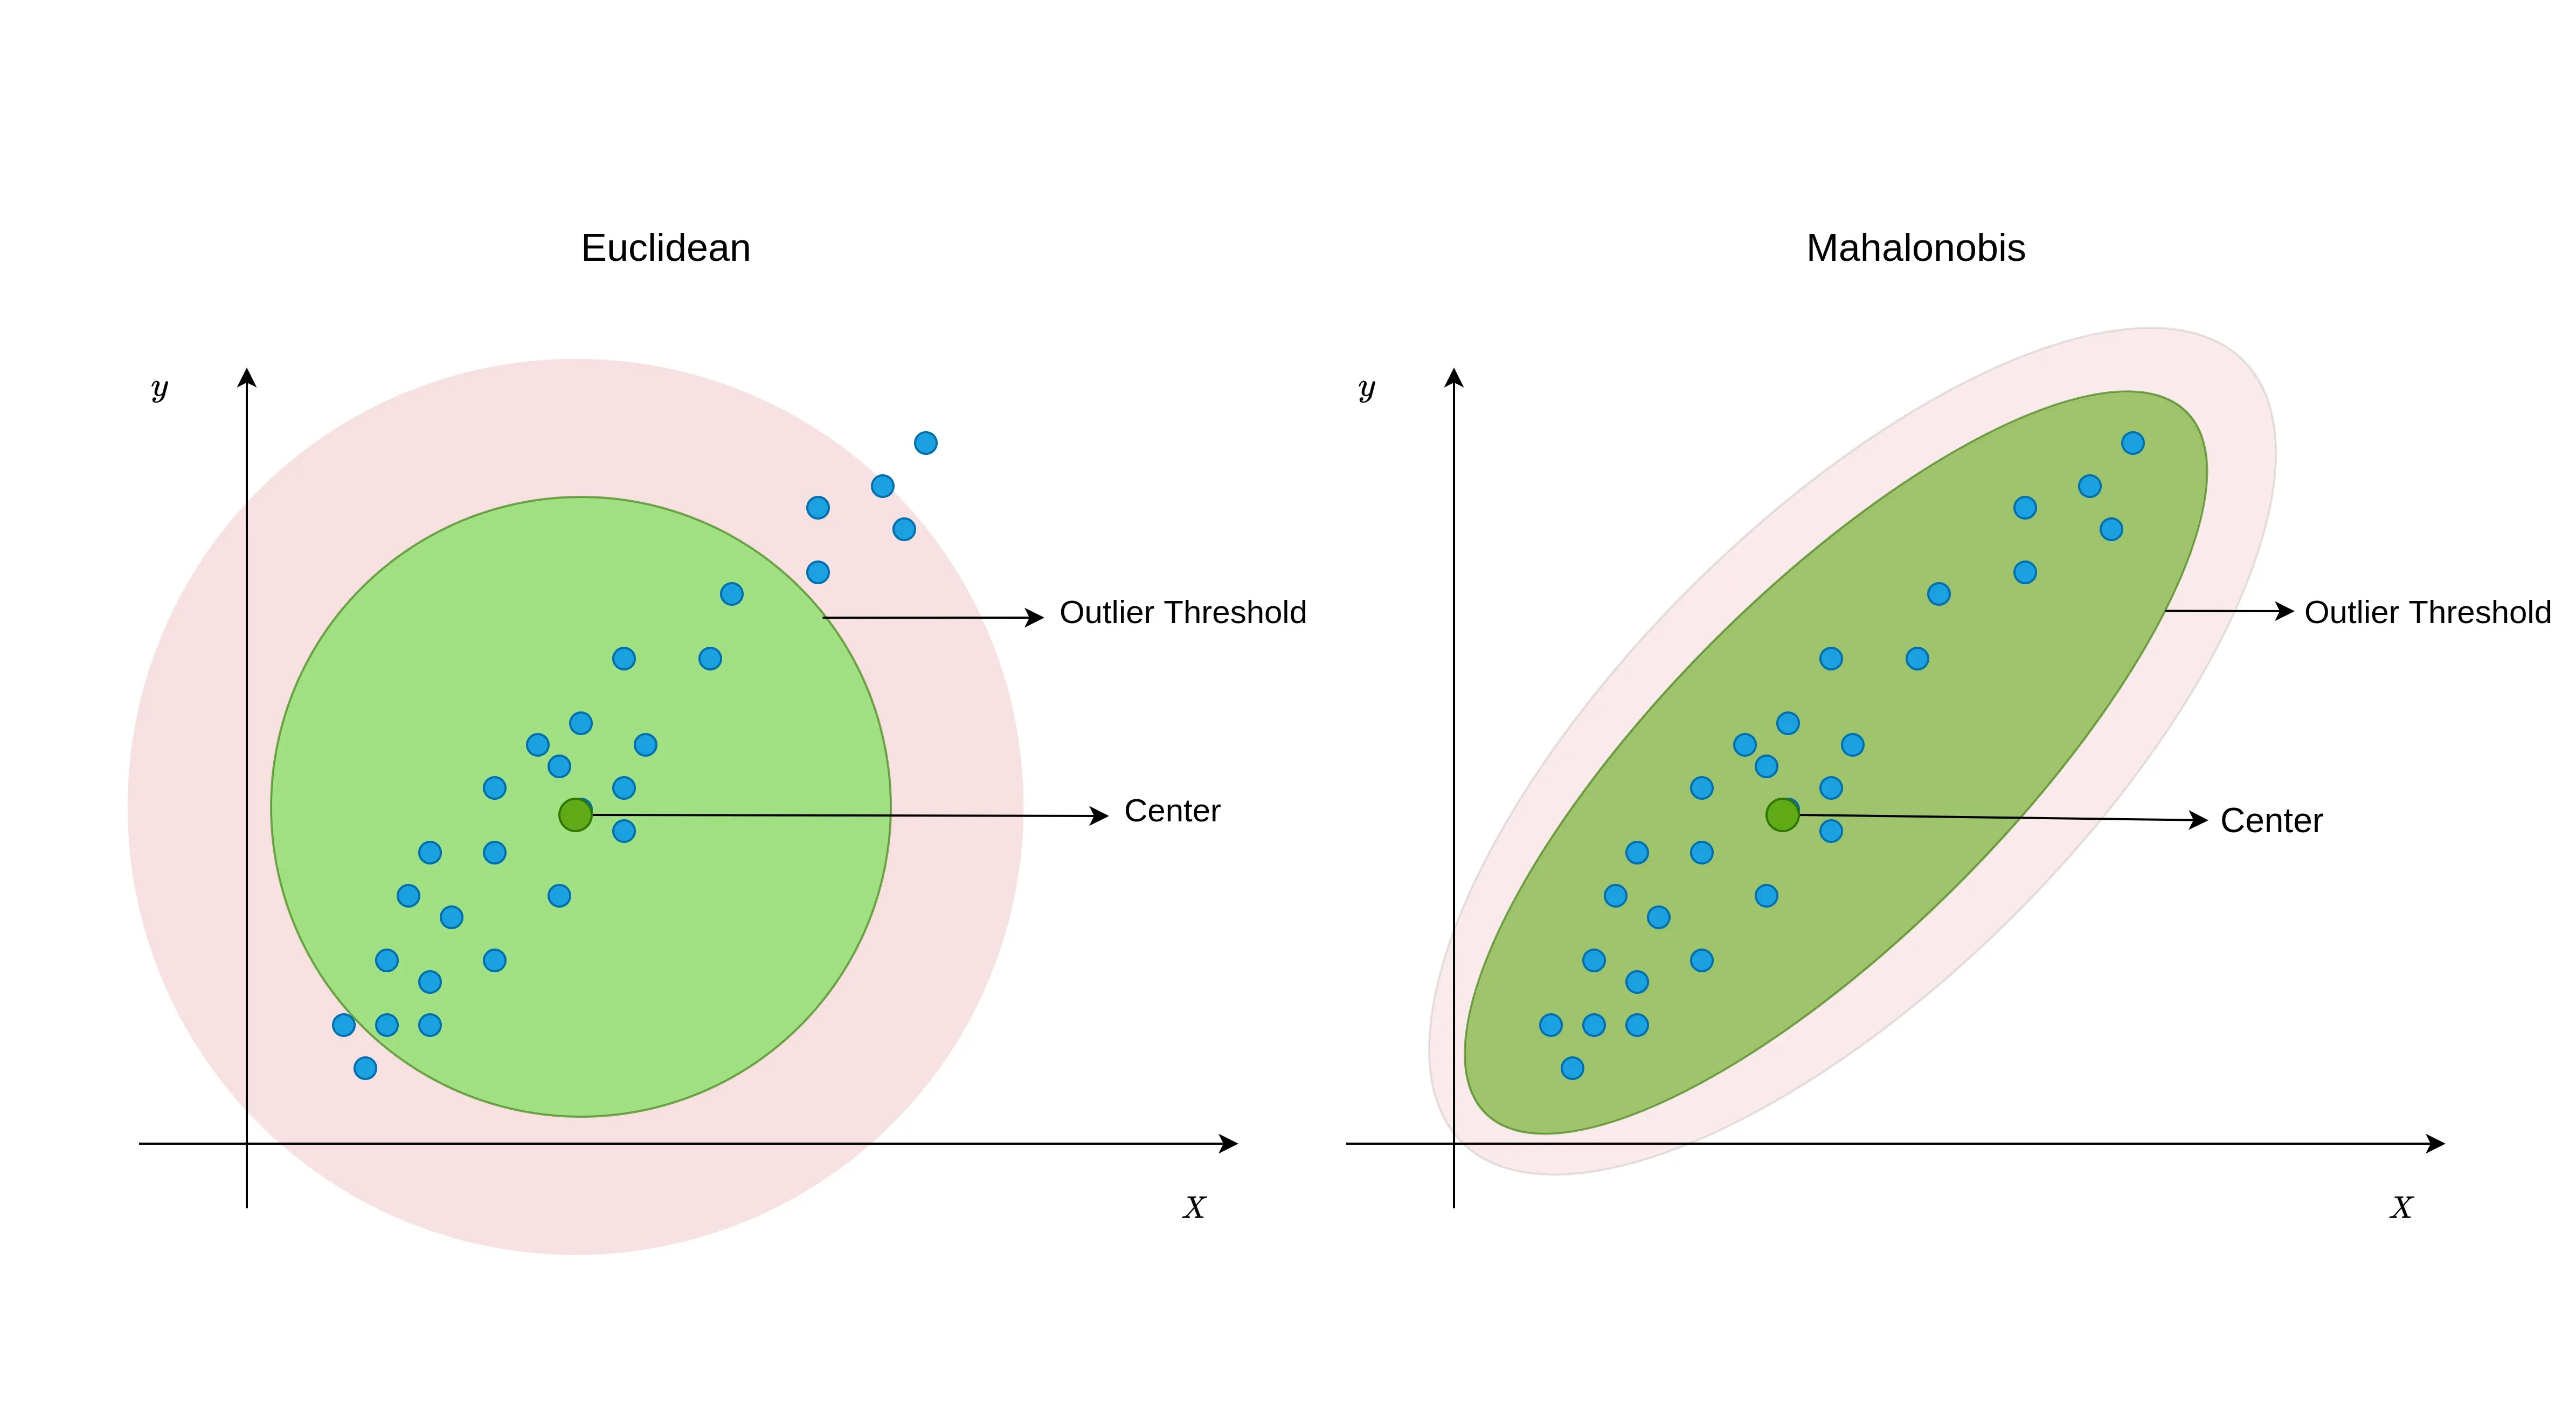
\includegraphics[width=0.9\linewidth]{Pictures/Optimizers/iSAM/Mahalanobis_Distance.png}
    \caption{Euclidean vs.\ Mahalanobis residual contours. \textit{Left:} isotropic (equal) weighting yields circular inlier regions. \textit{Right:} a covariance $\Sigma$ skews and scales the contours into an ellipse whose axes/tilt follow the noise correlations, whitening this with $\Sigma^{-1/2}$ maps this ellipse back to a circle.\textsuperscript{\cite{mahalanobis_distance_explained}}}
    \label{fig:mahalanobis-distance}
\end{figure}
\noindent
Mahalanobis distance is just ``error measured in the units of its noise'' (See Figure \ref{fig:mahalanobis-distance}). If a residual has high variance, it should be penalized less. If two components are correlated, they should not be treated as independent. That's what the covariance does. In the left plot (Euclidean), all directions are weighted equally so the inlier region is a circle. In the right plot (Mahalanobis), directions with low uncertainty are tighter and correlated axes tilt the ellipse. In SLAM cost function, each residual (process or measurement) is evaluated with its own covariance. Small reliable noises count more, whilst large noisy ones count less. When two parts of a measurement drift together, their error isn't along x or y alone, it's along some tilted direction. Mahalanobis tilts the ``penalty shape'' to match that direction. Penalties are smaller along noisy directions and larger where the sensor data is precise.
\\ \\
Equation \eqref{eq:optimizer-iSAM-delta-theta-star-mahalanobis-form} is a sum of Mahalanobis residuals (process terms use $\Lambda_i$, measurement terms use $\Gamma_k$). To turn that into one clean least squares system, first step is to ``whiten'' each residual so its noise is unit, for scalars divide by the standard deviation, for vectors apply the covariance's square root inverse to the residual and its Jacobians $\Sigma^{-1}$. After whitening, all errors are ordinary Euclidean ones, so the covariance symbols can be dropped, stack the Jacobians into one big sparse matrix $A$, stack the prediction errors into $b$, and solve the standard least squares problem \eqref{eq:optimizer-iSAM-delta-theta-star}.
\begin{equation}
    \Delta\theta^\star = \arg\min_{\Delta\theta}\; \|A\Delta\theta - b\|^2
    \label{eq:optimizer-iSAM-delta-theta-star}
\end{equation}
Here, $\theta$ stacks all unknowns (robot poses $x$ and landmarks $l$), $A$ is the single large, sparse (whitened) measurement Jacobian formed by stacking the block Jacobians $F, G, H,$ and $J$ from the linearized motion and measurement models, and $b$ is the stacked prediction error vector that collects the current odometry errors $a$ and measurement errors $c$ with a consistent sign convention. Intuitively, $A$ describes how residuals change for small state perturbations, $b$ encodes the present mismatch between predictions and measurements, and solving equation (\ref{eq:optimizer-iSAM-delta-theta-star}) yields the best local correction $\Delta\theta^\star$ used to update the estimate.
\\ \\
In the linearized setting, the optimal increment $\Delta\theta^\star$ is found by setting the gradient of the least squares objective to zero. This yields the normal equations according to iSAM paper \cite{iSAM_paper}:
$$
    A^{T}A\Delta\theta = A^{T}b
$$
Solving this system is typically performed using a numerically stable square root method (QR/Cholesky) rather than forming an explicit inverse. This gives the optimal correction $\Delta\theta^\star$. The state estimate is then updated as follows:
$$
    \theta \leftarrow \theta + \Delta\theta^\star
$$



\subsubsection{Incremental QR for fast updates (iSAM)}
The linearized SLAM subproblem is solved by least squares. Solving the normal equations $(A^\top A)\Delta\theta = A^\top b$ with Cholesky can be fast but very unstable and ill conditioned as the problem grows (it squares the condition number and increases fill in). iSAM avoids this by working directly with the whitened Jacobian $A$ using QR factorization, and by updating that factorization incrementally when new factors arrive.
\\ \\
Batch square root form (QR on the Jacobian) can be shown in iSAM paper \cite{iSAM_paper} to be of form:

$$
    A \;=\; Q
    \begin{bmatrix}
    R\\[2pt]
    0
    \end{bmatrix},
    \qquad Q^\top Q = I,
    \qquad R \text{: upper triangular}
$$
$$
    \begin{bmatrix}
    d\\ e
    \end{bmatrix}
    \;=\;
    Q^\top b
$$
$$
    \|A\Delta\theta - b\|^2
    \;=\;
    \|R\Delta\theta - d\|^2 + \|e\|^2
$$

\noindent
The iSAM paper \cite{iSAM_paper} shows that after QR the equation is:
$$
    A\Delta\theta - b \;=\;
    \begin{bmatrix} R \\ 0 \end{bmatrix}\Delta\theta -
    \begin{bmatrix} d \\ e \end{bmatrix},
    \quad\Rightarrow\quad
    \|A\Delta\theta - b\|^2 = \|R\Delta\theta - d\|^2 + \|e\|^2.
$$
\noindent
Put simply, once QR factorization is performed, the error splits into two parts. To make the total error as small as possible, set the first term to zero and solve:
\begin{equation}
    R\Delta\theta^\star = d
    \label{eq:optimizer-iSAM-fast-solution}
\end{equation}

\noindent
leaving $\|e\|^2$ as the (minimal) residual norm. If $R$ has full rank, this linearized system has one singular unique solution $\Delta\theta^\star$.
\\ \\
In iSAM the matrix $R$ is upper triangular, so equation (\ref{eq:optimizer-iSAM-fast-solution}) is solved by back substitution (no matrix inverse). This gives a fast, numerically stable way to compute the correction and update the state $\theta \leftarrow \theta + \Delta\theta^\star$ without heavy compute.



\subsubsection{What is R? The square root information matrix}
At the end of QR, the triangular factor $R$ satisfies the following form:
$$
R^\top R \;=\; A^\top A .
$$
This means $A^\top A$ (the information matrix obtained by linearization) is represented by the ``square root'' $R$. Working with $R$ keeps all the curvature of the problem but in a form that is easier to use and numerically safer because $R$ is upper triangular, so computations reduce to cheap substitution methods instead of expensive matrix inverses. Uncertainty can also be extracted directly from $R$. The state covariance is given by:
$$
\Sigma \;=\; (A^\top A)^{-1} \;=\; (R^\top R)^{-1},
$$
A dense inverse is never built. In reality, when entries of the uncertainty $\Sigma$ are needed, solve small triangular systems with $R^\top$ and $R$, and read only the pose blocks and the pose to landmark blocks of interest. Since $R$ is sparse and triangular, this is fast and stable, and it avoids forming $A^\top A$. (See \ref{sssec:iSAM-data-association} \nameref{sssec:iSAM-data-association})



\subsubsection{Matrix Factorization for building QR (Givens rotations)}
Here \emph{Givens rotations} is used to build an upper triangular factor $R$ from the (whitened) Jacobian $A$ by zeroing entries below the diagonal, one at a time. This yields a QR factorization without forming $A^\top A$ and without explicitly storing $Q$.
\\ \\
A Givens rotation is a $2\times 2$ orthogonal transform applied to two rows (or two columns) to annihilate one chosen entry. Givens rotation matrix is defined as:
\begin{equation}
    G(\varphi) =
    \begin{bmatrix}
        \cos\varphi & \sin\varphi \\
        -\sin\varphi & \cos\varphi
    \end{bmatrix}
    \label{eq:optimizer-iSAM-givens-rotation}
\end{equation}
Start at the leftmost non zero column of the $A$ matrix and sweep to the right, one column at a time. In each column, pick two rows, \textit{``k''} (the current pivot row) and \textit{``i''} (a row below it), and apply the small ``rotate and combine'' equation (\ref{eq:optimizer-iSAM-givens-rotation}) so the entry under the diagonal in that column becomes zero. Only those two rows are mixed, the new row \textit{``k''} becomes a bit of the old row \textit{``k''} plus a bit of row \textit{``i''}, and the new row \textit{``i''} becomes a bit of the old row \textit{``i''} minus a bit of row \textit{``k''}. Repeat down the column until all subdiagonal entries are gone, then move to the next column on the right. (see Figure \ref{fig:givens-rotation} down bellow for a visual of one Givens step)
\\ \\
As the algorithm sweeps the columns of $A$, the matrix is transformed into the upper triangular form, this is $R$, and the full $Q$ doesn't need to be formed to get to the result. Apply the same row rotations to $b$ as you eliminate entries so the right hand side stays consistent. After the initial factorization of $A$ matrix, new measurements don't require rebuilding $A$. Later it is shown that new whitened rows can be appended beneath the current $R$, then a short sequence of row rotations re-triangularizes $R$. In other words, updates operate directly on $R$ and $b$, and $A$ is bypassed for incremental steps.
\begin{figure}[H]
    \centering
    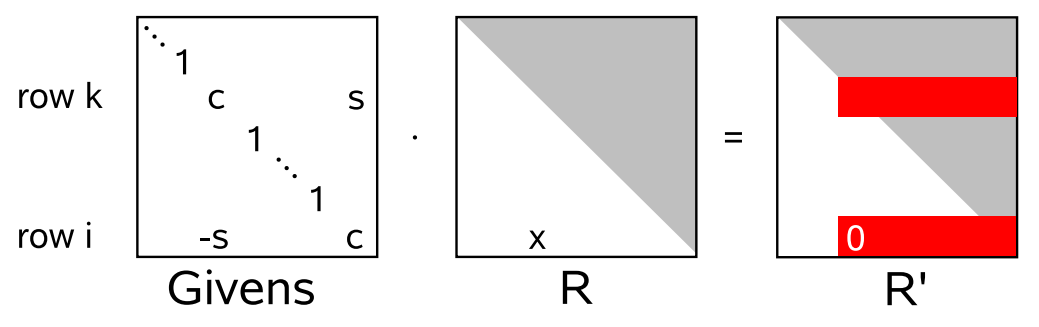
\includegraphics[width=0.9\linewidth]{Pictures/Optimizers/iSAM/Givens_Rotations.png}
    \caption{One Givens step in QR. The entry marked ``x'' is eliminated by rotating two rows, only the entries shown in red are modified, and the exact pattern depends on sparsity. Repeating this column wise (left to right) turns the matrix into an upper triangular $R$. Apply the same rotation to the $b$ vector to keep the least squares system consistent.\textsuperscript{\cite{iSAM_paper}}}
    \label{fig:givens-rotation}
\end{figure}
\noindent
In order to make $R$ upper triangular, $\varphi$ value must be chosen precisely to zero out a single sub diagonal entry in preliminary matrix, either be it $A$ matrix on batch step or $R$ matrix on iterative steps. The rotation angle $\varphi$ is computed from the two entries in the current column, the pivot $x=a_{kk}$ and the subdiagonal $y=a_{ik}$.
$$
    \begin{aligned}
        r=\sqrt{x^2+y^2}=\sqrt{a_{kk}^2+a_{ik}^2} \\
        c=\cos\varphi=\frac{x}{r}=\frac{a_{kk}}{r} \\
        s=\sin\varphi=\frac{y}{r}=\frac{a_{ik}}{r} 
    \end{aligned}
$$
Solving for $\varphi$ gives the following answer, where $\alpha = x = a_{kk}$ and $\beta = y = a_{ik}$:
\begin{equation}
    (\cos\varphi,\ \sin\varphi)=
    \begin{cases}
    (1,\,0), & \text{if }\beta=0,\\[6pt]
    \left(-\dfrac{\alpha}{\beta}\,\dfrac{1}{\sqrt{1+(\alpha/\beta)^2}},\ \dfrac{1}{\sqrt{1+(\alpha/\beta)^2}}\right), & \text{if }|\beta|>|\alpha|,\\[10pt]
    \left(\dfrac{1}{\sqrt{1+(\beta/\alpha)^2}},\ -\dfrac{\beta}{\alpha}\,\dfrac{1}{\sqrt{1+(\beta/\alpha)^2}}\right), & \text{otherwise.}
    \end{cases}
    \qquad\text{with }\ \alpha:=a_{kk},\ \beta:=a_{ik}.
    \label{eq:optimizer-iSAM-givens-rotation-find-phi}
\end{equation}
These coefficients in equation \eqref{eq:optimizer-iSAM-givens-rotation-find-phi} give the same rotation as \eqref{eq:optimizer-iSAM-givens-rotation}. 

Givens rotations guarantee that the $(i,k)$ entry of the working matrix becomes zero, and they preserve lengths. First the two numbers $[x,\,y]^\top$ are rotated. When embedded in the full matrix, the same rotation is applied to the affected parts of the two rows and to the matching entries of $b$. In practice, embed $G_{(i,k)}(\varphi)$ so it acts only on rows $k$ and $i$, and apply the same rotation to $b$ to keep the least squares system consistent.



\subsubsection{Incremental Updating}
\begin{figure}[H]
    \centering
    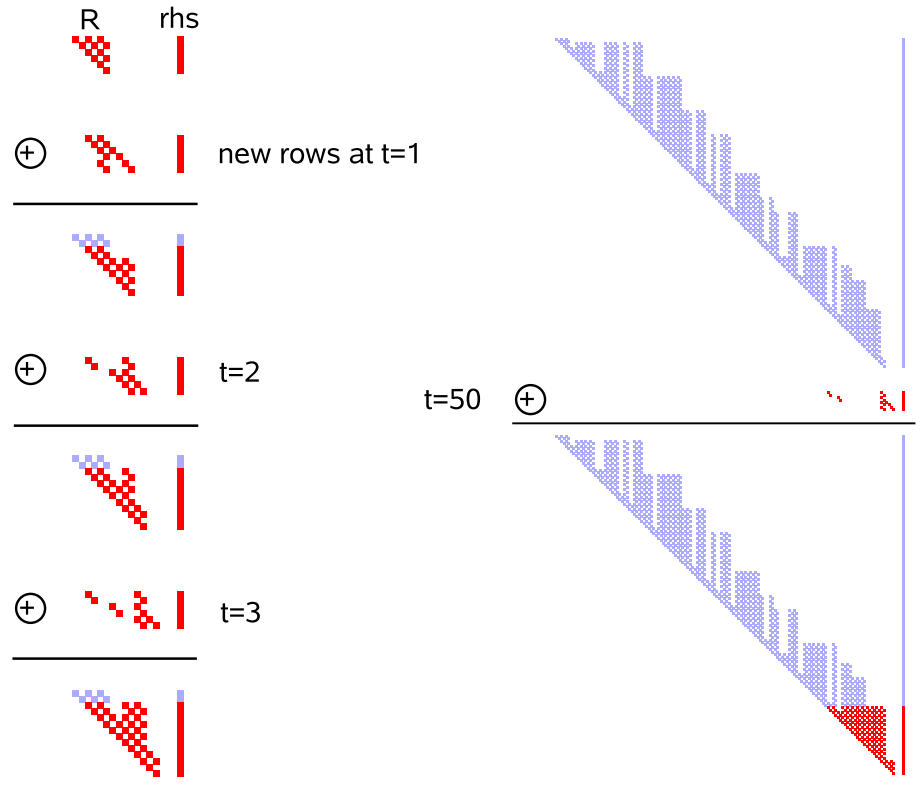
\includegraphics[width=0.5\linewidth]{Pictures/Optimizers/iSAM/R_Matrix_Update_Step.png}
    \caption{Incremental update of the factored system. A new whitened row $w^\top$ and RHS (Right Hand Side) entry $\gamma$ are appended beneath the current $R$ and $d$. A short sequence of Givens rotations restores the upper triangular form, yielding updated $R'$ and $d'$. Unchanged entries are shown in light color, only a small stencil is touched each step, so update cost stays bounded.\textsuperscript{\cite{iSAM_paper}}}
    \label{fig:R-matrix-update-step}
\end{figure}
\noindent
After the initial QR factorization, maintain the solution in ``square root'' form, an upper triangular matrix $R$ and a transformed right hand side $d$. Here, $R$ is the triangular factor that satisfies $R^\top R = A^\top A$ (the Gauss Newton information), and $d$ is the top part of $Q^\top b$. When a new measurement arrives, first whiten it (divide by its standard deviation or apply the square root information of its covariance) so it has unit variance. The whitened measurement contributes a new row $w^\top$ to the Jacobian and a new scalar $\gamma$ to the RHS (Right Hand Side). Notice that $A$ is NOT rebuild. Instead, append $w^\top$ under the current $R$, and $\gamma$ under the current $d$, which produces a system that is ``almost'' triangular but has one non triangular row at the bottom.
$$
    R' = \begin{bmatrix} R\\ w^\top \end{bmatrix},\qquad
    d' = \begin{bmatrix} d\\ \gamma \end{bmatrix}
$$
Next, re-triangularize locally with Givens rotations \eqref{eq:optimizer-iSAM-givens-rotation}. Only touching the columns where the new whitened Jacobian row $w^\top$ has nonzeros (i.e, the variables that this new factor actually connects to, such as a pose $x_i$ or a landmark $l_j$). Starting from the leftmost such column, each rotation mixes the current pivot row with the new bottom row to kill one sub diagonal entry. Repeat the process until the entire bottom row is zero and the matrix is upper triangular again. The equation would look something like this:
$$
    \begin{bmatrix} R\\ w^\top \end{bmatrix}
    \ \xrightarrow{\ \text{Givens rotation on affected columns}\ }\ 
    \begin{bmatrix} R'\\ 0 \end{bmatrix}
$$
While the matrix is rotates, apply the same rotations to the right hand side so that the least squares system stays consistent. Here $d$ is the transformed RHS (Right Hand Side) before the update and $\gamma$ is the new whitened RHS entry that pairs with $w^\top$. After the rotations, the top block becomes the updated RHS $d'$ used for solving, and the final bottom entry becomes a small leftover error $e_{\text{new}}$ that adds to the total residual. 
$$
    \begin{bmatrix} d\\ \gamma \end{bmatrix}
    \ \xrightarrow{\ \text{same rotations}\ }\ 
    \begin{bmatrix} d'\\ e_{\text{new}} \end{bmatrix}
$$
Intuitively, the new row $w^\top$ is ``folded up'' into the triangular structure by a short chain of 2x2 rotations that only touch the connected variables, everything else is left alone. Then get the correction by a fast back substitution on the updated matrix $R'$ and vector $d'$:
$$
    R'\Delta\theta^\star = d'
$$



\subsubsection{Loop Closure}
\begin{figure}[H]
    \centering
    % ---------- Left column ----------
    \begin{minipage}[t]{0.48\linewidth}
        \vspace{0pt}
        % Top-left (image 1)
        \begin{subfigure}[t]{\linewidth}
            \centering
            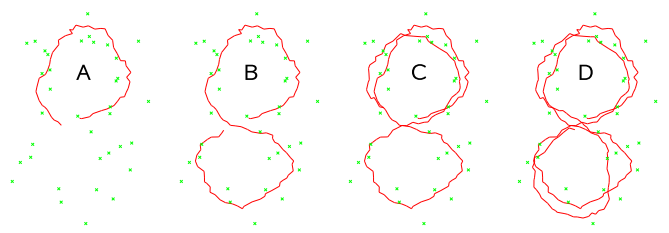
\includegraphics[width=\linewidth,height=0.47\textheight,keepaspectratio]{Pictures/Optimizers/iSAM/Variable_Reordering1.png}
            \caption{Simulated double 8 loop at key loop closure moments.\textsuperscript{\cite{iSAM_paper}}}\label{fig:l-top}
        \end{subfigure}\vspace{4pt}

        % Bottom-left row: (2) and (3) side-by-side
        \begin{subfigure}[t]{0.49\linewidth}
            \centering
            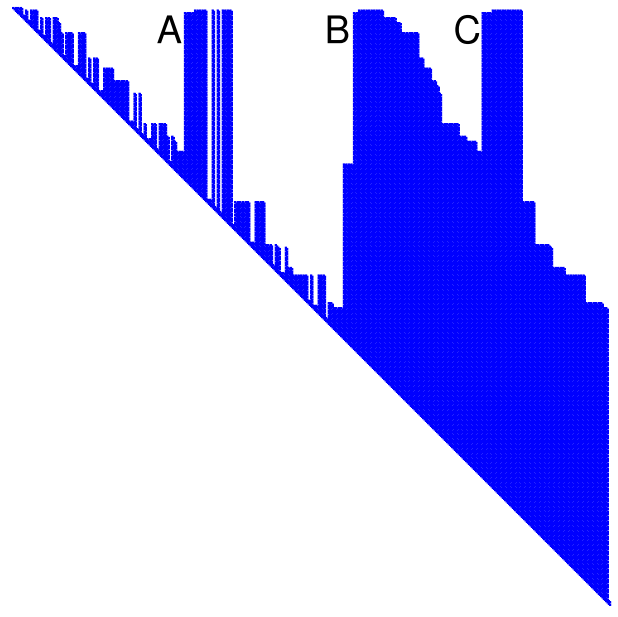
\includegraphics[width=\linewidth,height=0.20\textheight,keepaspectratio]{Pictures/Optimizers/iSAM/Variable_Reordering2.png}
            \caption{Upper triangular factor $R$ after several closures shows fill-in.\textsuperscript{\cite{iSAM_paper}}}\label{fig:l-bot-left}
        \end{subfigure}\hfill
        \begin{subfigure}[t]{0.49\linewidth}
            \centering
            
\includegraphics[width=\linewidth,height=0.20\textheight,keepaspectratio]{Pictures/Optimizers/iSAM/Variable_Reordering3.png}
            \caption{The same $R$ after variable reordering (COLAMD) becomes sparser again.\textsuperscript{\cite{iSAM_paper}}}\label{fig:l-bot-right}
        \end{subfigure}
    \end{minipage}\hfill
    % ---------- Right column ----------
    \begin{minipage}[t]{0.49\linewidth}
        \vspace{0pt}
        \begin{subfigure}[t]{\linewidth}
            \centering
            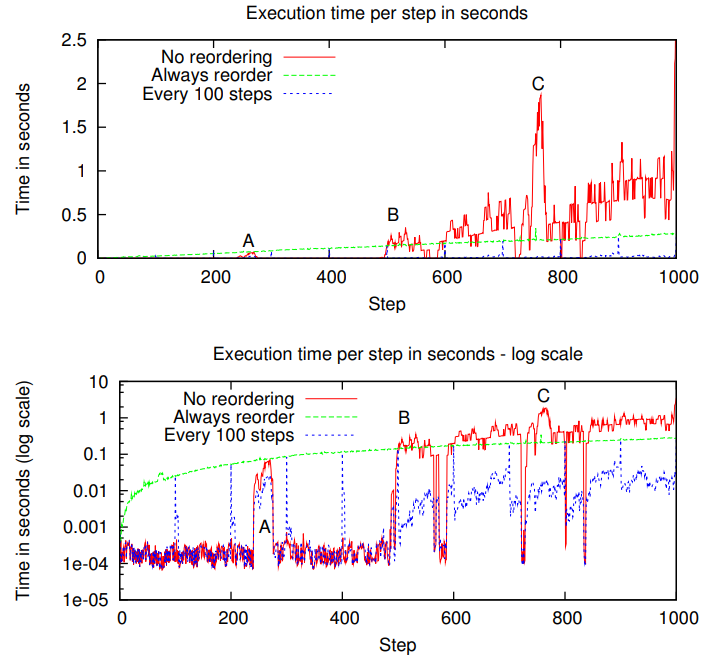
\includegraphics[width=\linewidth,height=0.98\textheight,keepaspectratio]{Pictures/Optimizers/iSAM/Variable_Reordering4.png}
            \caption{Per step execution time for three strategies. A: no reordering, B: reorder every step, C: reorder every 100 steps, shown in linear (top) and log (bottom) scale. Periodic reordering (C) limits spikes and keeps runtime predictable between loop closures.\textsuperscript{\cite{iSAM_paper}}}\label{fig:r-full}
        \end{subfigure}
    \end{minipage}

    \caption{Effect of loop closures and variable reordering (iSAM).\textsuperscript{\cite{iSAM_paper}}}
    \label{fig:variable-reordering}
\end{figure}
\noindent
Loop closures tie together far-apart parts of the trajectory (and landmarks), which makes previously separate columns interact. In QR terms this creates fill-in, R gets extra non zeros, so updates, back substitution, and selected covariance queries get slower and memory grows. This can be fixed by variable reordering. The goal is to pick a new elimination order that preserves sparsity. In practice run a heuristic like COLAMD (Column Approximate Minimum Degree) (often the block version for pose/landmark blocks) on the Jacobian's sparsity matrix $A$, then do batch factorization on the whole $A$ matrix using rotations \eqref{eq:optimizer-iSAM-givens-rotation} with that order \cite{iSAM_paper}. Reordering costs time because the factor must be rebuilt with a new permutation, but it pays back by making subsequent updates cheap again.
\\ \\
Because reordering is expensive, it is not done at every step. Instead, reordering is performed periodically every N steps (eks, 50 - 200) so the cost stays predictable. In marine AUV and ASV runs this keeps compute bounded. Between reorders incremental updates are fast and local. After a loop closure, one spike occurs (reorder + refactor), then the system returns to low latency. Practical tips when doing this step is to keep poses as blocks (block COLAMD) to reduce fill-in, align reordering with planned relinearization passes, and monitor simple stats (nonzeros in R, update time) to decide when N is too small (wasting time reordering) or too large (letting fill in snowball).  



\subsubsection{Re-Linearization}
Re-linearization keeps the local model valid. The QR and update methods assume the system is locally linear around the current estimate, but with angles, three dimensional motion, and nonlinear sensor data, that approximation drifts as the robot moves. If it is not refreshed, increments grow, the optimizer biases the map, and loop closures can fail. The remedy is to re-linearize and recompute Jacobians at the current state for the factors that matter. Doing this for every factor at every step is too expensive, so in practice new factors are always linearized, and older ones are refreshed only when needed.
\\ \\
In iSAM the practical schedule is to run incremental updates between maintenance cycles, then perform a full re-linearization every N steps. Between cycles, old factors are not re-linearized, new factors are whitened and inserted, and $R$ is updated incrementally. At the cycle boundary after N steps, the entire problem is re-linearized at the current estimate, the full Jacobian $A$ is rebuilt conceptually, variables are reordered with COLAMD to restore sparsity, and the system is refactored using equation \eqref{eq:optimizer-iSAM-givens-rotation} to obtain a fresh triangular $R$. For this reason variable reordering is usually grouped with batch re-linearization at the same N step.
\\ \\
$N$ must be chosen carefully, by balancing freshness vs compute. If N is too large, the linearization point drifts far from reality, Jacobians no longer match the true geometry, corrections become biased, loop closures pull hard, and the map can warp (a classic ``stale linearization'' issue). If $N$ is too small, the system stops often to re-linearize and refactor, wasting CPU and power, and reducing real-time throughput.



\subsubsection{Data Association from R}\label{sssec:iSAM-data-association}
For data association, Mahalanobis based approach is often used instead of plain nearest neighbour Approach. Nearest neighbour measures raw Euclidean distance and ignores sensor noise and correlations. Mahalanobis measures the innovation in the units of its uncertainty, so noisy directions count less, precise directions count more, and correlated components are handled correctly (See Figure \ref{fig:mahalanobis-distance}). For a candidate match between current pose $x_i$ and landmark $l_j$, form the innovation $\nu_k$ and score:
$$
    d_k^2=\nu_k^\top\,\Xi_k^{-1}\,\nu_k,\qquad
    \Xi_k=J_k\,\Sigma\,J_k^\top+\Gamma_k
$$
\noindent
where $J_k=[\,H^{x_i}\ \ H^{l_j}\,]$ is the linearized measurement Jacobian, $\Gamma_k$ is the sensor noise, and $\Sigma$ is the state covariance. 
\\ \\
This type of data association often uses gating with a chi-square test. The test keeps matches that are within $d_k^2\le \chi^2_{m,\alpha}$ (right dimension $m$, chosen confidence $\alpha$). From the survivors, pick the ``minimum cost'' one (or solve a global assignment using $d_{ij}^2$ as the cost matrix if several features compete). One thing to note about this approach is that the full dense $\Sigma=(R^\top R)^{-1}$ is not required for data association, only the local covariances influenced by the measurement. These covariances can be extracted directly from the square root information matrix $R$. Pose blocks and pose to landmark blocks are available online as well. Landmark terms on the other hand are either a approximate fast conservative estimate or computed exactly on demand. This keeps the association real-time for the most part.
Here are the partitioned forms.
Full state covariance (poses vs. landmarks):
$$
    \Sigma \;=\;
    \begin{bmatrix}
    \Sigma_{xx} & \Sigma_{xL}\\[4pt]
    \Sigma_{Lx} & \Sigma_{LL}
    \end{bmatrix}
$$
\noindent
where $\Sigma_{xx}$ is pose to pose, $\Sigma_{LL}$ is landmark to landmark, and $\Sigma_{xL}=\Sigma_{Lx}^\top$ is pose to landmark.
\\ \\
The $2\times2$ submatrix needed for a single candidate $(x_i,l_j)$:
$$
\Sigma_{\{x_i,l_j\}} \;=\;
\begin{bmatrix}
\Sigma_{x_i x_i} & \Sigma_{x_i l_j}\\[4pt]
\Sigma_{l_j x_i} & \Sigma_{l_j l_j}
\end{bmatrix}
$$
\noindent
\textbf{Fast marginals from the square root factor (online/live)} 
\\ \noindent
In iSAM paper \cite{iSAM_paper}, they propose keeping the current pose last in the ordering. Then the covariances needed for association, the pose variance $\Sigma_{x_i x_i}$ and the pose to landmark cross terms $\Sigma_{x_i l_j}$ come straight from the square root factor $R$ with two small triangular solves:
$$
    R^\top Y = B,\qquad R X = Y
$$
where $B=\begin{bmatrix}0\\ I_{d_x}\end{bmatrix}$ simply selects the last pose block of size $d_x$. Because $R$ is upper triangular and $B$ is zero above the last block, the forward solve gives:
$$
Y=\big[\,0,\ldots,0,\ R_{ii}^{-1}\,\big]^\top
$$
This $Y$ preliminary matrix is the clue, where only $d_x$ back substitutions are needed to get full $X$ vector. Reading the result $X$ yields, in one pass:
$$
\Sigma_{x_i x_i} \;\; \text{(bottom–right block of } \Sigma)\qquad
\Sigma_{l_j x_i}=\Sigma_{x_i l_j}^\top \;\; \text{for connected } l_j
$$
Intuitively ``solve up'' then ``solve down'' on $R$ for the last pose, and get exactly the columns of $\Sigma=(R^\top R)^{-1}$ that matter for gating in data association. This can be done every step without forming any dense inverses, only using $R$ square root information matrix iteratively. (See Figure \ref{fig:substitution-foward-backwards})
\begin{figure}[H]
  \centering
  \begin{subfigure}[t]{0.49\linewidth}
    \centering
    
\includegraphics[width=\linewidth]{Pictures/Optimizers/iSAM/Substitution_Forward.png}
    \caption{$R^\top Y = B$ (forward substitution). Sweep ``down'' the matrix to form $Y$ from a selector $B$ that picks the last pose block.}
    \label{fig:left}
  \end{subfigure}\hfill
  \begin{subfigure}[t]{0.49\linewidth}
    \centering
    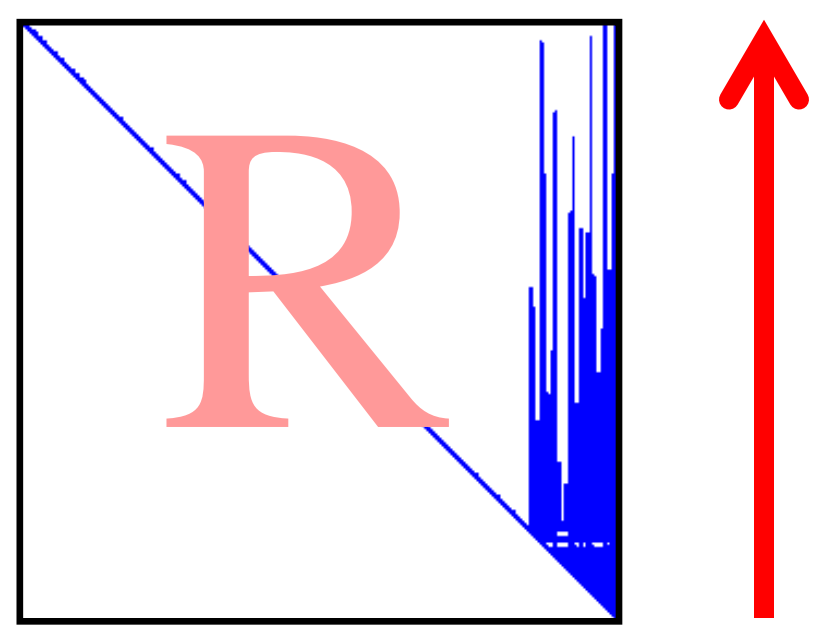
\includegraphics[width=\linewidth]{Pictures/Optimizers/iSAM/Substitution_Downwards.png}
    \caption{$R X = Y$ (back substitution). Sweep ``up'' the matrix to obtain the desired columns $X=\Sigma_{:\,,x_i}$ (pose and pose to landmark).}
    \label{fig:right}
  \end{subfigure}
  \caption{Grab the needed covariances in two quick steps: first solve ``down'' with $R^\top$, then solve ``up'' with $R$. Only touch entries near the last pose block, so each update stays fast and cheap.\textsuperscript{\cite{iSAM_paper}}}
  \label{fig:substitution-foward-backwards}
\end{figure}
\noindent
\textbf{Conservative landmark covariances (online/live)} 
\\ \noindent
Exact landmark landmark blocks $\Sigma_{jj}$ (or old pose to landmark $\Sigma_{(i-n)j}$) are expensive to extract at every step. Therefore in iSAM paper \cite{iSAM_paper} they propose using a safe, conservative bound built from the current pose covariance and the measurement noise via the linearized back projection:
$$
    \tilde\Sigma_{jj}
    \;=\;
    \bar J\,
    \begin{bmatrix}
    \Sigma_{ii} & 0\\[2pt]
    0 & \Gamma
    \end{bmatrix}
    \bar J^\top
$$
where $\bar J$ is the Jacobian of the local inverse measurement model, $\Sigma_{ii}$ is the current pose covariance, and $\Gamma$ is the measurement noise. This upper bounds landmark uncertainty (never over confident), is fast, and works well for online Mahalanobis gating. As more measurements of a landmark arrive, this bound typically tightens.
\\ \\
An important caveat to mention is that the true $\Gamma$ (measurement noise) is usually unknown. The iSAM recipe is to choose $\Gamma$ conservatively so the algorithms doesn't get overly confident. That keeps things safe but can make the gate too tight, causing the data association to reject more matches than it should. Later, a more reliable way to approximate $\Gamma$ from measurement characteristics is described. It avoids overconfidence and uses cues such as sonar range and resolution and landmark confidence, so the gate is realistic and not risky.
\\ \\
\textbf{Exact landmark covariances (on demand)} 
\\ \noindent
When accuracy is needed (eks: on risky loop closure, conflicting hypotheses), Data Association can recover exact $\Sigma_{jj}$ and $\Sigma_{(i-n)j}$ without forming the full dense inverse information matrix $\Sigma=(A^{T}A)^{-1}=(R^{T}R)^{-1}$. Because the covariance is the inverse of the information matrix:
$$
    \Sigma=(R^\top R)^{-1}, \qquad R^\top R\,\Sigma = I
$$
Needed entries can be extracted without forming the full inverse by solving for two triangular matrixes:
$$
R^\top Y = I, \qquad R \Sigma = Y
$$
The solve uses only the ``nonzero'' entries of $R$, so computation touches only the parts that matter, not the whole matrix. iSAM walks backwards along those non zero links and gives us exactly the covariance numbers $\sigma_{ij}$ Data Association ask for. If $R$ is mostly banded, this is near linear time. This exact method should only be used when its really needed (eks: a few $\Sigma_{jj}$ blocks to check on a loop closure). It's slower than the conservative shortcut, but still much faster than inverting the whole matrix.
\\ \\
\textbf{Alternative way to finding $\Gamma$} 
\\ \noindent
There's another angle. Instead of being very conservative with $\Gamma$ measurement noise. Uncertainty used in Data Association should reflect the sensor, for example a sonar for scanning the sea floor. With sonar the measurement noise can grow with range, and the transducer resolution can set per axis variances $N(0, \Sigma_{sonar})$. The landmark detection can also contribute its own uncertainty $N(0, \Sigma_{landmark})$. In practice these are combined to form the prediction uncertainty for the residual that is scored. In that case the effective covariance is:
$$
    \Gamma = Var(h(x, l)) = \Sigma_{sonar} + \Sigma_{landmark}
$$
This can be more informative than a one size fits all setting. However, this approach requires care. If the noise terms are too confident, the data association gate becomes too tight, matches become brittle, and the system can become unstable. Nevertheless, it often yields more accurate maps and a better estimate of the robot's track.



\subsubsection{Algorithm}
At each time step absorb new information, linearize around the current estimate, solve a small least squares, and update. Periodically refresh linearization and variable order. Concretely:
\begin{enumerate}
    \item \textbf{Add factors (whiten first):} take the new odometry/measurements and add them to the graph. ``Whiten”'' them so every residual has unit noise (as described before \eqref{eq:optimizer-iSAM-delta-theta-star}).

    \item \textbf{Linearize at the current guess \(\theta\):} turn the nonlinear motion/measurement models into local linear ones using the Jacobians in
    \eqref{eq:optimizer-iSAM-linearized-odometry} and \eqref{eq:optimizer-iSAM-linearized-measurement}. This gives the summed Mahalanobis cost \eqref{eq:optimizer-iSAM-delta-theta-star-mahalanobis-form}, which after whitening becomes one least squares problem \eqref{eq:optimizer-iSAM-delta-theta-star}.

    \item \textbf{Keep a triangular system up to date (QR):} append the new (whitened) rows and apply a few Givens rotations \eqref{eq:optimizer-iSAM-givens-rotation} so the matrix stays upper triangular $R$. Update the right hand side $b$ vector the same way (see ``Incremental Updating'').

    \item \textbf{Solve for the small change:} because $R$ is triangular, solve
    \eqref{eq:optimizer-iSAM-fast-solution} by back substitution (fast) to get the correction .

    \item \textbf{Update the estimate:} replace the old state with the improved one,
    $\theta \leftarrow \theta + \Delta\theta^\star$.

    \item \textbf{Every \(N\) steps (maintenance):} refresh accuracy by re-linearizing all factors at the new $\theta$, reorder variables (eks: COLAMD algorithm) to keep things sparse, and refactor with Givens \eqref{eq:optimizer-iSAM-givens-rotation} to get a clean $R$.

    \item \textbf{Data Association update:} read the needed covariances from $R$ (pose and pose to landmark live, landmark blocks conservative or exact on demand) and run Mahalanobis gating in Data Association for next matches.
\end{enumerate}



\subsubsection{Limitations}
iSAM is fast between updates but has practical downsides. They come from the ``data structure'', not the underlying SLAM algorithm. iSAM keeps a single, global square root information matrix $R$ (from $A^\top A$) and does periodic maintenance (reordering + re-linearization). This makes updates simple, but couples cost to global structure and variable ordering instead of just local changes.
\begin{itemize}
    \item \textbf{Latency spikes at maintenance:} Periodic global variable reordering and re-linearization trigger stalls (especially after loop closures), since $R$ must be refactored end to end.

    \item \textbf{Fill in growth between reorders:} Incremental QR on a fixed order accumulates fill in in $R$, touching more entries per update and increasing time/memory step by step.

    \item \textbf{All or nothing re-linearization:} iSAM typically refreshes many factors at maintenance even if most variables barely moved, wasting Jacobian recomputations.

    \item \textbf{Global refactor on ordering changes:} Any change to elimination order implies a large refactor of the global $R$, regardless of how small the new information is.

    \item \textbf{Broad marginal queries are costly:} Last pose and nearby cross terms can be pulled quickly from $R$, but wide $\Sigma$ blocks (eks: many landmarks or older poses) require multiple triangular solves and can be costly.

    \item \textbf{Schedule sensitivity:} Choosing ``every $N$ steps'' for reorder/re-linearize is heuristic, too small wastes time, too large lets fill in and linearization error grow, causing jitter and warp in the map.

    \item \textbf{Numerical robustness vs simplicity:} Working with $A$ and $R$ avoids explicit $A^\top A$, but long incremental runs plus fill in can still hurt conditioning and stability if ordering lags.
\end{itemize}
\noindent
These limitations motivated \textbf{iSAM2}, which replaces the single monolithic $R$ that is very static, with a Bayes tree representation that is dynamic and updates only the affected parts. We address iSAM2 and how it mitigates the issues above in the next chapter.

 \clearpage
\subsection{iSAM2}
iSAM2 stuff here \clearpage
\subsection{GTSAM}
GTSAM stuff here \clearpage

 \clearpage

% Refrences
\newpage
\printbibliography

\end{document}
% Document (STSTOPART) ==================================================

